% Options for packages loaded elsewhere
\PassOptionsToPackage{unicode}{hyperref}
\PassOptionsToPackage{hyphens}{url}
%
\documentclass[
]{article}
\usepackage{amsmath,amssymb}
\usepackage{lmodern}
\usepackage{iftex}
\ifPDFTeX
  \usepackage[T1]{fontenc}
  \usepackage[utf8]{inputenc}
  \usepackage{textcomp} % provide euro and other symbols
\else % if luatex or xetex
  \usepackage{unicode-math}
  \defaultfontfeatures{Scale=MatchLowercase}
  \defaultfontfeatures[\rmfamily]{Ligatures=TeX,Scale=1}
\fi
% Use upquote if available, for straight quotes in verbatim environments
\IfFileExists{upquote.sty}{\usepackage{upquote}}{}
\IfFileExists{microtype.sty}{% use microtype if available
  \usepackage[]{microtype}
  \UseMicrotypeSet[protrusion]{basicmath} % disable protrusion for tt fonts
}{}
\makeatletter
\@ifundefined{KOMAClassName}{% if non-KOMA class
  \IfFileExists{parskip.sty}{%
    \usepackage{parskip}
  }{% else
    \setlength{\parindent}{0pt}
    \setlength{\parskip}{6pt plus 2pt minus 1pt}}
}{% if KOMA class
  \KOMAoptions{parskip=half}}
\makeatother
\usepackage{xcolor}
\usepackage[margin=1.0in]{geometry}
\usepackage{longtable,booktabs,array}
\usepackage{calc} % for calculating minipage widths
% Correct order of tables after \paragraph or \subparagraph
\usepackage{etoolbox}
\makeatletter
\patchcmd\longtable{\par}{\if@noskipsec\mbox{}\fi\par}{}{}
\makeatother
% Allow footnotes in longtable head/foot
\IfFileExists{footnotehyper.sty}{\usepackage{footnotehyper}}{\usepackage{footnote}}
\makesavenoteenv{longtable}
\usepackage{graphicx}
\makeatletter
\def\maxwidth{\ifdim\Gin@nat@width>\linewidth\linewidth\else\Gin@nat@width\fi}
\def\maxheight{\ifdim\Gin@nat@height>\textheight\textheight\else\Gin@nat@height\fi}
\makeatother
% Scale images if necessary, so that they will not overflow the page
% margins by default, and it is still possible to overwrite the defaults
% using explicit options in \includegraphics[width, height, ...]{}
\setkeys{Gin}{width=\maxwidth,height=\maxheight,keepaspectratio}
% Set default figure placement to htbp
\makeatletter
\def\fps@figure{htbp}
\makeatother
\setlength{\emergencystretch}{3em} % prevent overfull lines
\providecommand{\tightlist}{%
  \setlength{\itemsep}{0pt}\setlength{\parskip}{0pt}}
\setcounter{secnumdepth}{-\maxdimen} % remove section numbering
\newlength{\cslhangindent}
\setlength{\cslhangindent}{1.5em}
\newlength{\csllabelwidth}
\setlength{\csllabelwidth}{3em}
\newlength{\cslentryspacingunit} % times entry-spacing
\setlength{\cslentryspacingunit}{\parskip}
\newenvironment{CSLReferences}[2] % #1 hanging-ident, #2 entry spacing
 {% don't indent paragraphs
  \setlength{\parindent}{0pt}
  % turn on hanging indent if param 1 is 1
  \ifodd #1
  \let\oldpar\par
  \def\par{\hangindent=\cslhangindent\oldpar}
  \fi
  % set entry spacing
  \setlength{\parskip}{#2\cslentryspacingunit}
 }%
 {}
\usepackage{calc}
\newcommand{\CSLBlock}[1]{#1\hfill\break}
\newcommand{\CSLLeftMargin}[1]{\parbox[t]{\csllabelwidth}{#1}}
\newcommand{\CSLRightInline}[1]{\parbox[t]{\linewidth - \csllabelwidth}{#1}\break}
\newcommand{\CSLIndent}[1]{\hspace{\cslhangindent}#1}
\usepackage{upgreek}
\usepackage{booktabs}
\usepackage{longtable}
\usepackage{graphicx}
\usepackage{array}
\usepackage{multirow}
\usepackage{wrapfig}
\usepackage{float}
\usepackage{colortbl}
\usepackage{pdflscape}
\usepackage{tabu}
\usepackage{threeparttable}
\usepackage{threeparttablex}
\usepackage[normalem]{ulem}
\usepackage{makecell}
\usepackage{setspace}
\doublespacing
\usepackage[left]{lineno}
\linenumbers
\modulolinenumbers
\usepackage{helvet}
\renewcommand*\familydefault{\sfdefault}
\usepackage[T1]{fontenc}
\usepackage[shortcuts]{extdash}
\usepackage[document]{ragged2e}
\usepackage{booktabs}
\usepackage{longtable}
\usepackage{array}
\usepackage{multirow}
\usepackage{wrapfig}
\usepackage{float}
\usepackage{colortbl}
\usepackage{pdflscape}
\usepackage{tabu}
\usepackage{threeparttable}
\usepackage{threeparttablex}
\usepackage[normalem]{ulem}
\usepackage{makecell}
\usepackage{xcolor}
\ifLuaTeX
  \usepackage{selnolig}  % disable illegal ligatures
\fi
\IfFileExists{bookmark.sty}{\usepackage{bookmark}}{\usepackage{hyperref}}
\IfFileExists{xurl.sty}{\usepackage{xurl}}{} % add URL line breaks if available
\urlstyle{same} % disable monospaced font for URLs
\hypersetup{
  hidelinks,
  pdfcreator={LaTeX via pandoc}}

\author{}
\date{\vspace{-2.5em}}

\begin{document}

\raggedright

\hypertarget{rarefaction-is-currently-the-best-approach-to-control-for-uneven-sequencing-effort-in-amplicon-sequence-analyses}{%
\section{Rarefaction is currently the best approach to control for
uneven sequencing effort in amplicon sequence
analyses}\label{rarefaction-is-currently-the-best-approach-to-control-for-uneven-sequencing-effort-in-amplicon-sequence-analyses}}

\vspace{20mm}

\textbf{Running title:} Use rarefaction

\vspace{20mm}

Patrick D. Schloss\({^\dagger}\)

\vspace{40mm}

\({\dagger}\) To whom correspondence should be addressed:

\href{mailto:pschloss@umich.edu}{pschloss@umich.edu}

Department of Microbiology \& Immunology

University of Michigan

Ann Arbor, MI 48109

\vspace{20mm}

\textbf{Research article}

\newpage

\hypertarget{abstract}{%
\subsection{Abstract}\label{abstract}}

Considering it is common to find as much as 100-fold variation in the
number of 16S rRNA gene sequences found across samples in a study,
researchers need to control for the effect of uneven sequencing effort.
How to do this has become a contentious question. Some have argued that
rarefying or rarefaction is ``inadmissible'' because it omits valid
data. A number of alternative approaches have been developed to
normalize and rescale the data that purport to be invariant to the
number of observations. I generated community distributions based on 12
published datasets where I was able to assess the ability of multiple
methods to control for uneven sequencing effort. Rarefaction was the
only method that could control for variation in uneven sequencing effort
when measuring commonly used alpha and beta diversity metrics. Next, I
compared the false detection rate and power to detect true differences
between simulated communities with a known effect size using various
alpha and beta diversity metrics. Although all methods of controlling
for uneven sequencing effort had an acceptable false detection rate when
samples were randomly assigned to two treatment groups, rarefaction was
consistently able to control for differences in sequencing effort when
sequencing depth was confounded with treatment group. Finally, the
statistical power to detect differences in alpha and beta diversity
metrics was consistently the highest when using rarefaction. These
simulations underscore the importance of using rarefaction to normalize
the number of sequences across samples in amplicon sequencing analyses.

\hypertarget{importance}{%
\subsection{Importance}\label{importance}}

Sequencing 16S rRNA gene fragments has become a fundamental tool for
understanding the diversity of microbial communities and the factors
that affect their diversity. Due to technical challenges, it is common
to observe wide variation in the number of sequences that are collected
from different samples within the same study. However, the diversity
metrics used by microbial ecologists are sensitive to differences in
sequencing effort. Therefore, tools are needed to control for the uneven
levels of sequencing. This simulation-based analysis shows that despite
a longstanding controversy, rarefaction is the most robust approach to
control for uneven sequencing effort. The controversy started because of
confusion over the definition of rarefaction and violation of
assumptions that are made by methods that have been borrowed from other
fields. Microbial ecologists should use rarefaction.

\newpage

\hypertarget{introduction}{%
\subsection{Introduction}\label{introduction}}

The ability to generate millions of 16S rRNA gene amplicon and
metagenomic sequence reads has allowed researchers to multiplex multiple
samples on the same sequencing run by pooling separate PCRs that can be
deconvoluted later based on index (aka barcode) sequences that are
embedded into the sequence of the PCR primers (1--3). Unfortunately, it
is common to observe variation in the number of sequence reads from each
sample vary by as much as 100-fold (e.g, see Figure S1). This occurs
because pooling of DNA from multiple PCRs is fraught with numerous
opportunities for technical errors to compound leading to a skewed
distribution. Aside from developing better methods of pooling DNA, the
question of how to control for uneven sequencing effort in microbial
ecology studies has become controversial.

The practice of rarefaction has been commonly used in ecology for more
than 50 years as a tool to control for uneven sequencing effort across
experimental replicates (4, 5). Microbial ecologists have used it to
compare 16S rRNA gene sequence data for the past 25 years (6--8). With
rarefaction the investigator selects a desired threshold of sequencing
effort and removes any samples below that threshold. They then randomly
select that many sequences, with replacement from each sample. Based on
the observed sequence counts, the researcher can then calculate alpha
diversity metrics including richness and diversity indices or beta
diversity metrics such as a Jaccard or Bray-Curtis dissimilarity index.
I refer to this single sampling as a subsample; this method is
implemented as the \texttt{sub.sample} function in mothur (9) and the
\texttt{rrarefy} function in the \texttt{vegan} R package (10).
Rarefaction repeats the subsampling a large number of times (e.g., 100
or 1,000 times) and calculates the mean of the alpha or beta diversity
metric over those subsamplings; rarefaction is implemented in mothur
using the \texttt{summary.single} and \texttt{dist.shared} functions (9)
and with the \texttt{vegan} R package using the \texttt{rarefy} or
\texttt{avgdist} functions (10). Rarefaction effectively tells a
researcher what an alpha or beta diversity metric would have been for a
collection of samples if they were all sequenced to the same depth.
Although a closed form equation exists to calculate the expected
richness (5), it is computationally easier to empirically calculate
richness and other alpha and beta diversity metrics by rarefaction.

In 2014, McMurdie and Holmes (11) announced that ``rarefying'' of
microbial community data was ``statistically inadmissible'' because it
omits valid data. In their simulations, they observed that rarefying
reduced the statistical power to correctly cluster samples into the same
treatment groups based on beta diversity metrics. Although the detail
was lost on many subsequent researchers, they did not describe
rarefaction, but rarefying (12). According to McMurdie and Holmes,
rarefying is a single subsampling of an OTU abundance table whereas
rarefaction repeats the subsampling step many times. Furthermore, their
simulations penalized the rarefied data by removing 15\% of the samples
and evaluated clustering quality using a clustering algorithm that
performed worse for rarefied data. According to my reanalysis of
rarefaction using the original simulation framework, rarefaction
outperformed other normalization method being used in 2014 for both
alpha and beta diversity metrics (12). Others have also critiqued the
original work (13). Regardless, there is a general sense in the
community that rarefying and rarefaction should not be used with
microbiome data.

Since McMurdie and Holmes published their simulations, others have
developed alternative approaches to control for uneven sequencing effort
in amplicon sequencing studies. For alpha diversity metrics, Willis used
toy datasets to demonstrate that one could estimate the richness for
each sample in a dataset and use those values for statistical
comparisons (14). Non-parametric estimators of richness and diversity
(15, 16) and parametric estimators of richness (17) have been used in
microbial ecology studies. For beta diversity metrics at least four
approaches have been pursued. First, one could use relative abundance
values where the observed number of sequences in an OTU is divided by
the total number of sequences in the sample (18). Second, normalization
strategies have been developed where the relative abundance is
multiplied by the size of the minimum desired sequencing effort and
fractional values are reapportioned to the OTUs to obtain integer values
(19, 20). Third, a variety of center log-ratio methods have been
developed where the compositional nature of the OTU counts is removed
and used to calculated Euclidean distances (aka Aitchison distances)
(18, 20--23). This strategy is purported to control for uneven
sequencing effort (22, 24); however, some have noticed that this feature
breaks down under certain conditions (25). Finally, as mentioned above,
variance stabilization transformations have been recommended to generate
values that can be used to calculate Euclidean distances (11).

The ongoing controversy over the use of rarefaction and the recent
development of alternative strategies to control for uneven sequencing
effort caused me to question how these methods compared to each other
using a simulation framework that overcame the issues with the McMurdie
and Holmes study. My analysis included 16S rRNA gene sequence data from
from 12 studies that characterized the variation in bacterial
communities from diverse environments (Table 1 and Figure S1). The
sequences were assigned to OTUs using a standard pipeline and their
frequencies and the number of sequences found in each sample were used
to generate simulated communities and treatment effects. For each
dataset and simulation, 100 replicate datasets were generated and used
as input to each of the strategies for controlling for uneven sequencing
effort. My overall conclusion was that rarefaction outperformed the
alternative strategies.

\hypertarget{results}{%
\subsection{Results}\label{results}}

\textbf{\emph{Without rarefaction, metrics of alpha diversity are
sensitive to sequencing effort.}} To test the sensitivity of various
approaches of measuring alpha diversity to sequencing effort, I
generated null models using OTU counts and sequencing depths from 12
studies. Under a null model, each community from the same dataset would
be expected to have the same alpha diversity regardless of the
sequencing effort. I measured the richness of the communities in each
dataset without any correction, using scaled ranked subsampling (SRS)
normalized OTU counts, with estimates based on non-parametric and
parametric approaches, and using rarefaction (e.g.~Figure S2). For each
dataset, all of the approaches, except for rarefaction, showed a strong
correlation between richness and the number of sequences in the sample
(Figure 1A). Next, I assessed diversity using the Shannon diversity
index and the inverse Simpson diversity index without any correction,
using normalized OTU counts, and rarefaction; I also used a
non-parametric estimator of Shannon diversity. The correlation between
sequencing depth and the diversity metric was not as strong as it was
for richness and the inverse Simpson diversity values were less
sensitive than the Shannon diversity values; however, the correlation to
the diversity metrics calculated with rarefaction were the lowest for
all of the metrics and studies (Figure 1A). The alpha-diversity metrics
calculated with rarefaction consistently demonstrated a lack of
sensitivity to sequencing depth.

\textbf{\emph{Without rarefaction, metrics of beta diversity are
sensitive to sequencing effort.}} To test the sensitivity of various
approaches of measuring beta diversity to sequencing effort, I used the
same null models used for studying the sensitivity of alpha diversity.
Under a null model, the ecological distance between any pair of samples
would be the same regardless of the difference in the number of
sequences observed in each sample (e.g., Figure S3). First, I calculated
the Jaccard distance coefficient between all pairs of communities within
a dataset. The Jaccard distance coefficient is the fraction of OTUs that
are unique to either community and does not account for the abundance of
the OTUs. Jaccard distances were calculated using the uncorrected OTU
counts, with rarefaction, relative abundances, and following
normalization using cumulative sum scaling (CSS) and SRS. Only the
distances calculated with rarefaction showed a lack of sensitivity to
sequencing effort (Figure 1B). Second, I analyzed the sensitivity of the
Bray-Curtis distance coefficient, which is a popular metric that
incorporates the abundance of each OTU. Similar to what I observed with
the Jaccard coefficient, only the data normalized with rarefaction
showed a lack of sensitivity to sequencing effort (Figure 1B). Third, I
calculated the Euclidean distance on raw OTU counts where the central
log-ratio (CLR) was calculated (i.e., Aitchison distances) by ignoring
OTUs in samples with zero counts (Robust CLR), adding a pseudo-count of
one to all OTU counts prior to calculating the CLR (One CLR), adding a
pseudo-count of one divided by the total number of sequences obtained
for the community (Nudge CLR), and imputing the value of zero counts
(Zero CLR). The Aitchison distances were all strongly sensitive to
sequencing effort (Figure 1B). Finally, I used the
variance-stabilization transformation (VST) from DESeq2 prior to
calculating Euclidean distances. Again, there was a strong sensitivity
to sequencing effort (Figure 1B). Although Euclidean distances are not
typically used on raw or rarefaction-normalized count data in ecology
(26), Euclidean distances calculated with rarefaction were not sensitive
to sequencing effort. Across each of the beta diversity metrics and
approaches used to account for uneven sequencing effort and sparsity,
rarefaction was the least sensitive approach to differences in
sequencing effort.

\textbf{\emph{Rarefaction limits the detection of false positives when
sequencing effort and treatment group are confounded.}} Next, I
investigated the impact of the various strategies and metrics on falsely
detecting a significant difference using the the same communities
generated from the null model in the analysis of alpha and beta
diversity metrics. To test for differences in alpha and beta diversity I
used the non-parametric Wilcoxon test and non-parametric
permutation-based multivariate analysis of variance (PERMANOVA). First,
I employed an unbiased null treatment model to measure the false
detection rate, which should not have meaningfully differed from 5\%.
Indeed, for each dataset and alpha and beta diversity metric and
strategy for accounting for uneven sequencing, approximately 5\% of the
tests yielded a significant result (Figure 2). Second, I employed a
biased null treatment model where the treatment group was completely
confounded with the number of sequences in each sample. Under this
model, only the data normalized with rarefaction consistently resulted
in a 5\% false positive rate for alpha and beta diversity metrics
(Figure 2). These results aligned with the observed sensitivity of alpha
and beta diversity metrics to sequencing effort and underscore the value
of rarefaction.

\textbf{\emph{Rarefaction preserves the statistical power to detect
differences between treatment groups.}} To assess the impact of
different approaches to control for uneven sequencing effort I performed
two additional simulations. In the first simulation, I implemented a
skewed abundance distribution model to create two treatment groups for
each dataset that were each populated with half of the samples each with
the same number of sequences as the samples had in the observed data.
The two treatment groups varied in their structure such that one had the
same abundances as the null distribution above and the other had 10\% of
its OTUs randomly selected to increase their counts by 5\%. The power to
detect differences in richness between the two simulated treatment
groups by all approaches was low (Figure 4A). This was likely because
the approach for generating the perturbed community did not necessarily
change the number of OTUs in each treatment group. Regardless, the
simulations testing differences in richness using the Rice and Stream
datasets had the greatest power when the richness data were calculated
with rarefaction. To explore this further, a richness-adjusted community
model was created by removing 3\% of the OTUs from a null model model.
As suggested by the first simulation, the richness data calculated with
rarefaction had a higher statistical power than the other approaches
when measuring richness (Figure 5). The simulations testing the power to
detect differences in Shannon diversity also showed that rarefaction
performed better than the other methods (Figure 4A). When testing for
differences in the Inverse Simpson diversity index the the difference
between rarefaction and the other methods was negligible (Figure 4A).
For tests of beta diversity I found that rarefaction was the most
reliable approach to maintain statistical power to detect differences
between two communities. Among the tests using the Jaccard and
Bray-Curtis metrics, raw count data and CSS normalized data had little
power relative to using rarefaction, relative abundance, and SRS to
normalize the uneven sequencing depths. The differences in power between
counts normalized with rarefaction, relative abundance, and SRS data was
small, but if there were differences, the power obtained using
rarefaction was greater than the other methods. Among the tests using
Euclidean distances, using raw counts and CLR and DESeq2 transformed
data had little power relative to the distances calculated using
rarefaction and relative abundances. This power-based analysis of the
simulated communities using different methods of handling uneven sample
sizes demonstrated the value of rarefaction for preserving the
statistical power to detect differences between treatment groups for
measures of alpha and beta diversity.

\textbf{\emph{Increased rarefaction depth reduces intra-sample variation
in alpha and beta diversity.}} Once concern with using rarefaction is
the perceived loss of sequencing information when a large fraction of
data appears to be removed when the community with the greatest
sequencing depth is sampled to the size of the community with the least
(e.g., the smallest sample in the Bioethanol dataset had 1.04\% of
sequences that were in the largest sample). To assess the sensitivity of
alpha and beta diversity metrics to rarefaction depth, I again used the
dataset generated using the null models, but used rarefaction with each
community to varying sequencing depths (Figure 6). The richness values
increased with sequencing effort as rare OTUs would continue be
detected. In contrast, the Shannon diversity and Bray-Curtis values
plateaued with increased sequencing effort. This result was expected
since increased sequencing would lead to increased precision in the
measured relative abundance of the OTUs. Next, I measured the
coefficient of variation (i.e., the mean divided by the standard
deviation) between samples for richness, Shannon diversity, and
Bray-Curtis distances. Although the mean richness appeared to increased
unbounded with sequencing effort, the coefficient of variation for each
dataset was relatively stable. In general, the coefficient of variation
increased slightly with sequencing depth only to decline once smaller
samples were removed from the analysis at higher sequencing depths.
Interestingly, the coefficient of variation between Shannon diversity
values decreased towards zero with increased sequencing effort and the
coefficient of variation between Bray-Curtis distances tended to
increase. Regardless, the coefficients of variation were relatively
small. This analysis indicates that there are benefits to increased
sequencing depths.

\textbf{\emph{Most studies have a high level of sequencing coverage.}}
To explore the concern over loss of sequencing depth further, I
calculated the Good's coverage for the observed data. The median
coverage for each dataset ranged between 89.4 and 99.8\% for the
Seagrass and Human datasets, respectively (Figure 7). When I used a
rarefaction threshold with each dataset at the size of the smallest
community in the dataset, with the exception of the Seagrass, Rice, and
Stream datasets, the median coverage with rarefaction was still greater
than 90\%. These results suggest that most studies had a level of
sequencing coverage that aligned with the diversity of the communities.
Next, I used the null model for each dataset to ask how much sequencing
effort was required to obtain higher levels of coverage. To obtain 95
and 99\% coverage, an average of 2.70 and 101.20-fold more sequence data
was estimated to be required than was required to obtain 90\% coverage,
respectively (Figure 7). As suggested by the simulated coverages curve
in Figure 7, these estimates are conservative. Regardless, the
sequencing effort required to achieve higher sequencing depth would
likely limit the number of samples that could be sequenced when
controlling for costs. Although it may be disconcerting to use
rarefaction to normalize to a sequencing depth that is considerably
lower than that obtained for the best sequenced community in a dataset,
sequencing coverage for many environments is probably adequate even at
the lower sequencing depth. Of course, regardless of the concerns
surrounding the choice of the rarefaction depth, the results throughout
this study demonstrate that rarefaction is necessary to avoid reaching
incorrect inferences.

\hypertarget{discussion}{%
\subsection{Discussion}\label{discussion}}

Over the past decade, the question of whether to use rarefaction with
microbial community sequence data has become controversial. The analyses
I presented here strongly indicate that rarefaction is necessary to
control for uneven sequencing effort when comparing communities based on
alpha and beta diversity indices. Compared to all other methods,
rarefaction removed the correlation between sequencing depth and alpha
or beta diversity metrics when the sequencing depth varied by as much as
97-fold across samples. I showed that this correlation could lead
falsely detecting differences between treatment groups if sequencing
depth and sequencing effort are confounded. The correlation with
sequencing effort leads to an artificial increase in the variation
between samples and a reduced power to detect true differences in alpha
and beta diversity. For these reasons, rarefaction is a valuable tool to
control for uneven sequencing effort until improved statistical
procedures are developed or it becomes possible to more evenly
distribute sequencing effort across samples.

The primary alternative to rarefaction for measuring alpha diversity is
to estimate the metric using non-parametric or parametric models with
raw counts and to then compare the estimates (7, 14). My results
demonstrate that such approaches are limited for several reasons. First,
non-parametric richness estimates such as ACE and Chao1 are sensitive to
sequencing effort. Therefore, these strategies do not, in practice,
remove the effects of sequencing effort. Second, parametric approaches,
such as those implemented in the \texttt{breakaway} R package, generate
confidence intervals that are likely to include the true richness and
theoretically shrink with increased sequencing effort. Yet for most
samples, the confidence intervals around the estimates are too wide to
be meaningful, again leading to an inability to remove the effects of
sequencing effort. Third, it has become an increasingly common practice
for researchers to remove sequences that are rare in a sample (e.g.,
those that appear once). Although that approach was not taken in this
study, removing rare sequences would skew the distribution of sequences
and OTUs leading to a distortion of the measurement of alpha diversity
(27). The effects of removing rare sequences would vary across samples
depending on the number of sequences in each sample. One interesting
result of this analysis was the demonstration that as metrics that
depend less on rare taxa are used, the effect of uneven sequencing
effort was reduced. For example, richness counts a sequence appearing
once as much as sequence appearing 1,000 times, while the Shannon
diversity index places more emphasis on the more abundant sequence, and
the inverse Simpson index even more. Although normalizing communities to
a common number of sequences is also suggested (e.g., SRS normalization)
to control for uneven sequencing effort, the current analysis indicates
that its performance does not meet that of rarefaction. For analysis of
alpha diversity metrics, rarefaction is the most effective and
consistent approach to control for uneven sequencing effort.

Use of relative abundances, normalized counts, variance stabilizing
transformations, and centered log ratios have each been recommended as
more robust alternatives to rarefaction. Again, the only approach that
consistently removed the effects of uneven sequencing effort was
rarefaction. Most of the recommendations borrow techniques from methods
for identifying differential gene expression. Unfortunately, there is an
important but under appreciated difference between gene expression and
community data. This is the interpretation of unobserved data. For gene
expression analysis in a single organism the lack of any sequencing data
for a gene would indicate that although the gene was present, its
expression was below the limit of detection. Sequencing the same
organism under multiple conditions would not lead to a seemingly
unbounded number of genes in the organisms. Rather, the number of genes
has a definite limit that is knowable from the genome sequence. With
microbiome data, an unobserved sequence could mean that the organism was
present, but below the limit of detection or that the organism was
missing. Because we have yet to exhaustively sample any community in the
same way we have sequenced a single genome, it is unreliable to impute
the presence of all organisms. Yet, this is exactly what the variance
stabilization transformation and most CLR techniques do. This analysis
has demonstrated a clear correlation between distances calculated by
these methods and sequencing effort. This result is at odds with the
claims by others that the distances are scale invariant (22, 24). Again,
rarefaction is the most effective and consistent approach to control for
uneven sequencing effort when calculating beta diversity metrics.

Two common critiques of rarefaction are that the approach omits valid
data and that the selection of rarefaction threshold is arbitrary (11).
I disagree with both critiques. All of the data are used to calculate
the mean value of the metrics after repeatedly subsampling the data.
When the dataset is subsampled, every sequence has a random chance of
being included in the calculated metric. When that subsampling is
repeated a large number of times (e.g., 100 or 1000) the risks of
ignoring or oversampling rare taxa are mitigated. Furthermore, it is
curious that the study making the original critique removed rare
sequences. A parallel analysis to this study has demonstrated that many
of these sequences are likely valid and that removal of rare sequences
can bias alpha and beta diversity metrics and reduce statistical power
(27). As for the second criticism, I would resist the claim that the
selection of the rarefaction threshold is arbitrary. In practice, there
is a tradeoff between sampling breadth and sequencing depth. Greater
breadth will increase the statistical power to compare treatment groups
and greater depth will increase the resolution to describe the
communities. My personal process for rarefaction threshold involves
looking for a natural break in the distribution of the number of
sequences. For example, the Lake dataset used in this study had a clear
break around 10,000 sequences (Figure S1). I would also consider what
samples are below any break that I select. If there were critical
samples below the break I would either reduce the threshold or obtain
more sequences from those samples. As shown in my analysis of Good's
coverage values, most studies obtain an ample level of coverage and
would need to increase their sequencing depth by 10-fold to increase the
coverage by several percentage points. In past work, I have favored
distributing the total number of sequences to increase sampling breadth
rather than sequencing depth.

The up to 100-fold difference in sample sizes is an unfortunate
byproduct of how sequencing libraries are constructed. Researchers
perform separate PCRs for each sample with unique index (aka, barcode)
sequences that allow them to later assign sequences back to the samples
that they came from. When the PCR products are pooled, efforts are taken
to pool the fragments in equimolar ratios. Researchers use one of two
approaches. First, they often will quantify the concentration of DNA
from each PCR and then pool DNA in the desired amounts. Alternatively,
they may use normalization plates where each well can hybridize a
uniform amount of DNA that is then eluted and pooled. Clearly, both
approaches have limitations that reduce the ability to truly achieve
equimolar mixture. In addition, for some samples it is common to
co-amplify non-specific DNAs which may add to the challenges of
achieving equimolar mixtures of the desired amplicons since those
sequences will be removed (28). Regardless, it is clear that better
strategies are needed to reduce the variation in the number of sequences
generated for each sample.

All simulations have weaknesses and should be interpreted with caution.
However, the simulated communities generated and analyzed in this study
had the advantage of being designed with known properties including the
alpha and beta diversity and the their differences between treatment
groups. Indeed, is is perfectly admissible and proper to use rarefaction
with microbial community data. The alternative is to risk reaching
unwarranted conclusions.

\hypertarget{materials-and-methods}{%
\subsection{Materials and Methods}\label{materials-and-methods}}

\textbf{Choice of datasets.} The specific studies used in this study
were selected because their data was publicly accessible through the
Sequence Read Archive, the original investigators sequenced the V4
region of the 16S rRNA gene using paired 250 nt reads, and my previous
familiarity with the data. The use of paired 250 nt reads to sequence
the V4 region resulted in a near complete two-fold overlap of the V4
region resulting in high quality contigs with a low sequencing error
rate (3). These data were processed through a standardized sequence
curation pipeline to generate operational taxonomic units (OTUs) using
the mothur software package (3, 9). OTUs were identified using the
OptiClust algorithm to cluster sequences together that were not more
than 3\% different from each other (29).

\textbf{Null community model.} Null community models were generated such
that within a dataset the number of sequences per sample and the number
of sequences per OTU across all samples within the dataset were the same
as was observed in original. This model effectively generated
statistical samples of a single community so that there should not have
been a statistical difference between the samples. This model
implemented by randomly assigning each sequence in the dataset to an OTU
and sample while keeping constant the number of sequences per sample and
the total number of sequences in each OTU. This is a similar approach to
that of the IS algorithm described by Ulrich and Gotelli (30). Because
the construction of the null models was a stochastic process, 100
replicates were generated for each dataset.

\textbf{Null treatment models.} I created an unbiased and biased
treatment model. In the unbiased model, samples were randomly assigned
to one of two treatment groups. In the biased treatment model, samples
that had more than the median number of sequences for a dataset were
assigned to one treatment group and the rest were assigned to a second
treatment group. Comparison of any diversity metric across the two
treatment groups should have only yielded a significant result in 5\% of
the simulations when testing under a Type I error (i.e., \(\alpha\)) of
0.05.

\textbf{Skewed abundance community model.} In the skewed abundance
community model, communities were randomly assigned to one of two
simulated treatment groups. Communities in the first treatment group
were generated by calculating the relative abundance of each OTU across
all samples and using those values as the probability of sampling each
OTU. This probability distribution was sampled, with replacement, until
each sample had the same number of sequences that it did in the observed
data. Samples in the second treatment group were generated by adjusting
the relative abundances of the OTUs in the firs treatment group by
increasing the relative abundance of 10\% of the OTUs by 5\%. These
values were determined after empirically searching for conditions that
resulted in a large fraction of the randomizations yielding a
significant result across most of the studies. Sequences were sampled
from the skewed community community until each sample had the same
number of sequences that it did in the observed data. Under the skewed
abundance community model, each sample represented a statistical
sampling of two communities such that there should not have been a
statistically significant difference within a treatment group, but there
was between the treatment groups. Because the construction of the skewed
abundance community model was a stochastic process, 100 replicates were
generated for each dataset.

\textbf{Richness-adjusted community model.} In the richness-adjusted
community model, communities were randomly assigned to one of two
simulated treatment groups. Communities in the first treatment group
were generated by calculating the relative abundance of each OTU across
all samples and using those values as the probability of sampling each
OTU. This probability distribution was sampled until each sample had the
same number of sequences that it did in the observed data. Samples in
the second treatment group were generated by removing 3\% of the OTUs
from the dataset and recalculating the relative abundance of the
remaining OTUs. Sequences were sampled from the richness-adjusted
community distribtion, with replacement, until each sample had the same
number of sequences that it did in the observed data. Under the
richness-adjusted community model, each sample represented a statistical
sampling of two communities such that there should not have been a
statistically significant difference within a treatment group, but there
was between the treatment groups. Because the construction of the
richness-adjusted community model was a stochastic process, 100
replicates were generated for each dataset.

\textbf{Test of statistical significance.} Statistical comparisons of
alpha diversity metrics across the simulated treatment groups were
performed using the non-parametric two-sample Wilcoxon test as
implemented in \texttt{wilcoxon.test} in the \texttt{stats} base R
package. This test was selected because the alpha-diversity metrics
tended to not be normally distributed and each dataset required a
different transformation to normalize the data. Comparisons of beta
diversity metrics were performed using the \texttt{adonis2} function
from the \texttt{vegan} (v.2.6.2) R package (10). The \texttt{adonis2}
function implements a non-parametric multivariate analysis of variance
using distances matrices (31). Throughout this study I used 0.05 as the
threshold for assessing the statistical significance of any P-values.

\textbf{Power analysis.} The parameters used to design the skewed
abundance and richness-adjusted community models were set to impose a
known effect size when using community data normalized by rarefaction.
The statistical power to detect these differences was determined by
calculating the p-value for each of 100 replicate simulated set of
samples from each dataset using the various alpha and beta diversity
metrics. The percentage of tests that yielded a significant P-value was
considered the statistical power (i.e., 1 minus the Type II error) to
detect the difference.

\textbf{Alpha diversity calculations.} Various strategies for handling
uneven sequencing effort were evaluated to identify the best approach
for calculating community richness and Shannon and inverse Simpson
diversity indices. OTU counts were used as input to calculate sample
richness and Shannon and inverse Simpson diversity using mothur (9, 32).
Shannon diversity was calculated as

\[H_{shannon} = - \sum_{i=1}^{S_{obs}} \frac{n_i}{N} ln \frac{n_i}{N}\]

The Simpson diversity was calculated as

\[D_{simpson} = \frac {\sum_{i=1}^{S_{obs}} {n_i \left ( n_i - 1 \right )}}{N \left( N-1 \right )}\]

The inverse Simpson diversity was calculated as \(1/D_{simpson}\). In
both formulae, \(n_i\) was the number of sequences in OTU \(i\) and
\(N\) iwass the number of sequences in the sample. Rarefaction of
richness, Shannon diversity and Inverse Simpson diversity values were
carried out in mothur. Briefly, mothur calculates each value on a random
draw of the same number of sequences from each sample and obtains a mean
value based on 1,000 random draws. Scaled ranked subsampling (SRS) was
used to normalize OTU counts to the size of the smallest sample in each
dataset using the SRS R package (v.0.2.3)(19). Normalized OTU counts
were used to calculate sample richness and Shannon and inverse Simpson
diversity values using mothur. Data normalized by cumulative sum scaling
(CSS) were not reported for alpha-diversity values since the relative
abundances of the features do not change with the normalization
procedure (20). The non-parametric bias-corrected Chao1 and ACE richness
estimators (16) and a non-parametric estimator of the Shannon diversity
(15) were calculated using raw OTU counts with mothur. Parametric
estimates of sample richness were calculated using the
\texttt{breakaway} (BA) R package (v.4.7.9)(17). My analysis reports
both the results from running default model selection procedure and the
Poisson model. The default model selection returned either the Kemp,
Negative Binomial, or Poisson models. Relative abundance data were not
used to calculate alpha diversity metrics since the richness and
evenness does not change from the raw data when dividing each sample by
the total number of sequences in the sample.

\textbf{Beta diversity calculations.} Similar to the alpha diversity
calculations, multiple approaches were used to control for uneven
sequencing effort and calculate beta diversity. Raw and OTU counts were
used for input to calculate the Jaccard, Bray-Curtis, and Euclidean
dissimilarity indices using the \texttt{vegdist} function from the
\texttt{vegan} R package (v.2.6.2)(10). The Jaccard index was calculated
as

\[D_{Jaccard}=1-\frac{S_{AB}}{S_A+S_B-S_{AB}}\]

where \(S_A\) and \(S_B\) were the number of OTUs in samples \(A\) and
\(B\) and \(S_{AB}\) was the number of OTUs shared between the two
samples. The Bray-Curtis index was calculated as

\[D_{Bray-Curtis}=1-\frac{\sum_{i=1}^{S_T} \left| n_{A,i} - n_{B,i}\right| }{ N_A + N_B}\]

where \(n_{A,i}\) and \(n_{B,i}\) were the number of sequences observed
in OTU \(i\) from samples \(A\) and \(B\), respectively. \(N_A\) and
\(N_B\) were the total number of sequences in samples \(A\) and \(B\),
respectively. \(S_T\) was the total number of OTUs observed between the
two samples. The Euclidean distance was calculated as

\[D_{Euclidean}=1-\sqrt{\sum_{i=1}^{S_T}\left(n_{A,i} - n_{B,i}\right)^2}\]

These metrics were calculated using the relative abundance of each OTU
using the \texttt{vegdist} function from the \texttt{vegan} R package.
The relative abundance was calculated as the number of sequences in the
OTU (e.g., \(n_{A,i}\)) divided by the total number of sequences in the
sample (e.g., \(N_A\)).

Beta-diversity values generated with rarefaction were calculated using
the \texttt{avgdist} function in vegan. Briefly, \texttt{vegan}'s
\texttt{avgdist} function calculates each pairwise dissimilarity index
after obtaining a random draw of the same number of sequences from each
sample. After obtaining 100 random draws it returns the mean value.

Three approaches were taken to normalize the number of sequences across
samples within a dataset. Scaled ranked subsampling (SRS) and cumulative
sum scaling (CSS) were used to normalize raw OTU counts using the
\texttt{SRS} (v.0.2.3) and \texttt{metagenomeSeq} (v.1.36.0) R packages,
respectively (19, 20). The normalized counts were then used to calculate
Jaccard and Bray-Curtis dissimilarity indices. Finally, the
variance-stabilization transformation (VST) as implemented in the
\texttt{DESeq2} (v.1.34.0) R package was used to normalize the data as
described by McMurdie and Holmes (11, 33). Because the VST approach
generated negative values, which are incompatible with calculating
Jaccard and Bray-Curtis dissimilarity values, Euclidean distances were
calculated instead.

Raw OTU counts were used to calculate centered log ratio (CLR) values
for each OTU, which were then used to calculate Euclidean distances;
such distances are commonly referred to as Aitchison distances. CLR
abundances are calculated as:

\[
CLR\left(n_j\right) = \left[ \ln\frac{x_{ij}}{g(x_j)}, ..., \ln\frac{x_{S_Tj}}{g(x_j)}\right]
\]

where \(x_{ij}\) was the number of sequences observed for OTU \(i\) in
sample \(j\) and \(g()\) was the geometric mean, \(x_j\) was the count
of the \(S_T\) OTUs in sample \(j\). Because the geometric mean is zero
if any OTU is absent from a sample, the CLR is undefined when there are
unobserved OTUs in a sample. To overcome this problem, I attempted a
four approaches. The first, Zero CLR, imputed the value of the zeroes
based on the observed data using the zCompositions (v.1.4.0.1) R package
(34). The second, One CLR, added a pseudo-count of 1 to the abundance of
all OTUs (18, 20). The third, Nudge CLR, added a pseudo-count of 1
divided by the total number of sequences in a sample to each OTU in the
sample (18, 23). The final approach, Robust CLR, removed unobserved OTUs
prior to calculating the CLR (22).

\textbf{Analysis of sequencing coverage.} To assess the level of
sequencing coverage I calculated Good's coverage (\(C_{Good}\)) using
mothur:

\[C_{Good} = 100\% \times \left(1-\frac{n_1}{N_T} \right)\]

where \(n_1\) was the number of OTUs with only one sequence in the
sample and \(N_T\) was the total number of sequences in the sample.
Good's coverage was calculated using (i) the observed OTU counts for
each sample and dataset, (ii) following rarefaction (1,000 iterations)
of the observed OTU counts to the size of the smallest sample in each
dataset, and (iii) after rarefaction (1,000 iterations) of the null
community distribution.

\textbf{Reproducible data analysis.} A complete reproducible workflow
written in Snakemake (v.7.15.2) and Conda (v.4.12.0) computational
environment can be obtained from the GitHub hosted git repository for
this project
(\url{https://github.com/SchlossLab/Schloss_Rarefaction_XXXXX_2023}).
This paper was written in R-flavored markdown (v.2.16) with the
\texttt{kableExtra} (v.1.3.4) package. The mothur (v.1.47.0) and R
(4.1.3) software packages were used for all analyses with extensive use
of functions in the tidyverse metapackage (v.1.3.1). A preliminary
version of this analysis was presented as the Rarefaction video series
on the Riffomonas Project YouTube channel
(\url{https://www.youtube.com/playlist?list=PLmNrK_nkqBpJuhS93PYC-Xr5oqur7IIWf}).

\vspace{10mm}

\textbf{Acknowledgements.}

I am grateful to the researchers who generated the datasets used in this
study. I also thank the individuals who asked questions and commented on
the preliminary version of this project, which was released as a YouTube
playlist on the Riffomonas channel. This work was supported in part by
funding from the National Institutes of Health (U01AI124255,
P30DK034933, R01CA215574).

\newpage

\hypertarget{references}{%
\subsection{References}\label{references}}

\setlength{\parindent}{-0.25in}
\setlength{\leftskip}{0.25in}

\noindent

\hypertarget{refs}{}
\begin{CSLReferences}{0}{1}
\leavevmode\vadjust pre{\hypertarget{ref-Sogin2006}{}}%
\CSLLeftMargin{1. }%
\CSLRightInline{\textbf{Sogin ML}, \textbf{Morrison HG}, \textbf{Huber
JA}, \textbf{Welch DM}, \textbf{Huse SM}, \textbf{Neal PR},
\textbf{Arrieta JM}, \textbf{Herndl GJ}. 2006. Microbial diversity in
the deep sea and the underexplored {``}rare biosphere{''}. Proceedings
of the National Academy of Sciences \textbf{103}:12115--12120.
doi:\href{https://doi.org/10.1073/pnas.0605127103}{10.1073/pnas.0605127103}.}

\leavevmode\vadjust pre{\hypertarget{ref-Caporaso2010}{}}%
\CSLLeftMargin{2. }%
\CSLRightInline{\textbf{Caporaso JG}, \textbf{Lauber CL},
\textbf{Walters WA}, \textbf{Berg-Lyons D}, \textbf{Lozupone CA},
\textbf{Turnbaugh PJ}, \textbf{Fierer N}, \textbf{Knight R}. 2010.
Global patterns of 16S {rRNA} diversity at a depth of millions of
sequences per sample. Proceedings of the National Academy of Sciences
\textbf{108}:4516--4522.
doi:\href{https://doi.org/10.1073/pnas.1000080107}{10.1073/pnas.1000080107}.}

\leavevmode\vadjust pre{\hypertarget{ref-Kozich2013}{}}%
\CSLLeftMargin{3. }%
\CSLRightInline{\textbf{Kozich JJ}, \textbf{Westcott SL}, \textbf{Baxter
NT}, \textbf{Highlander SK}, \textbf{Schloss PD}. 2013. Development of a
dual-index sequencing strategy and curation pipeline for analyzing
amplicon sequence data on the {MiSeq} illumina sequencing platform.
Applied and Environmental Microbiology \textbf{79}:5112--5120.
doi:\href{https://doi.org/10.1128/aem.01043-13}{10.1128/aem.01043-13}.}

\leavevmode\vadjust pre{\hypertarget{ref-Sanders1968}{}}%
\CSLLeftMargin{4. }%
\CSLRightInline{\textbf{Sanders HL}. 1968. Marine benthic diversity: A
comparative study. The American Naturalist \textbf{102}:243--282.
doi:\href{https://doi.org/10.1086/282541}{10.1086/282541}.}

\leavevmode\vadjust pre{\hypertarget{ref-Hurlbert1971}{}}%
\CSLLeftMargin{5. }%
\CSLRightInline{\textbf{Hurlbert SH}. 1971. The nonconcept of species
diversity: A critique and alternative parameters. Ecology
\textbf{52}:577--586.
doi:\href{https://doi.org/10.2307/1934145}{10.2307/1934145}.}

\leavevmode\vadjust pre{\hypertarget{ref-Dunbar1999}{}}%
\CSLLeftMargin{6. }%
\CSLRightInline{\textbf{Dunbar J}, \textbf{Takala S}, \textbf{Barns SM},
\textbf{Davis JA}, \textbf{Kuske CR}. 1999. Levels of bacterial
community diversity in four arid soils compared by cultivation and 16S
{rRNA} gene cloning. Applied and Environmental Microbiology
\textbf{65}:1662--1669.
doi:\href{https://doi.org/10.1128/aem.65.4.1662-1669.1999}{10.1128/aem.65.4.1662-1669.1999}.}

\leavevmode\vadjust pre{\hypertarget{ref-Hughes2001}{}}%
\CSLLeftMargin{7. }%
\CSLRightInline{\textbf{Hughes JB}, \textbf{Hellmann JJ},
\textbf{Ricketts TH}, \textbf{Bohannan BJM}. 2001. Counting the
uncountable: Statistical approaches to estimating microbial diversity.
Applied and Environmental Microbiology \textbf{67}:4399--4406.
doi:\href{https://doi.org/10.1128/aem.67.10.4399-4406.2001}{10.1128/aem.67.10.4399-4406.2001}.}

\leavevmode\vadjust pre{\hypertarget{ref-Moyer1998}{}}%
\CSLLeftMargin{8. }%
\CSLRightInline{\textbf{Moyer CL}, \textbf{Tiedje JM}, \textbf{Dobbs
FC}, \textbf{Karl DM}. 1998. Diversity of deep-sea hydrothermal vent
archaea from loihi seamount, hawaii. Deep Sea Research Part {II}:
Topical Studies in Oceanography \textbf{45}:303--317.
doi:\href{https://doi.org/10.1016/s0967-0645(97)00081-7}{10.1016/s0967-0645(97)00081-7}.}

\leavevmode\vadjust pre{\hypertarget{ref-Schloss2009}{}}%
\CSLLeftMargin{9. }%
\CSLRightInline{\textbf{Schloss PD}, \textbf{Westcott SL},
\textbf{Ryabin T}, \textbf{Hall JR}, \textbf{Hartmann M},
\textbf{Hollister EB}, \textbf{Lesniewski RA}, \textbf{Oakley BB},
\textbf{Parks DH}, \textbf{Robinson CJ}, \textbf{Sahl JW}, \textbf{Stres
B}, \textbf{Thallinger GG}, \textbf{Horn DJV}, \textbf{Weber CF}. 2009.
Introducing mothur: Open-source, platform-independent,
community-supported software for describing and comparing microbial
communities. Applied and Environmental Microbiology
\textbf{75}:7537--7541.
doi:\href{https://doi.org/10.1128/aem.01541-09}{10.1128/aem.01541-09}.}

\leavevmode\vadjust pre{\hypertarget{ref-Dixon2003}{}}%
\CSLLeftMargin{10. }%
\CSLRightInline{\textbf{Dixon P}. 2003. {VEGAN}, a package of r
functions for community ecology. Journal of Vegetation Science
\textbf{14}:927--930.
doi:\href{https://doi.org/10.1111/j.1654-1103.2003.tb02228.x}{10.1111/j.1654-1103.2003.tb02228.x}.}

\leavevmode\vadjust pre{\hypertarget{ref-McMurdie2014}{}}%
\CSLLeftMargin{11. }%
\CSLRightInline{\textbf{McMurdie PJ}, \textbf{Holmes S}. 2014. Waste
not, want not: Why rarefying microbiome data is inadmissible. {PLoS}
Computational Biology \textbf{10}:e1003531.
doi:\href{https://doi.org/10.1371/journal.pcbi.1003531}{10.1371/journal.pcbi.1003531}.}

\leavevmode\vadjust pre{\hypertarget{ref-Schloss2023wnwn}{}}%
\CSLLeftMargin{12. }%
\CSLRightInline{\textbf{Schloss PD}. 2023. Waste not, want not:
Revisiting the analysis that called into question the practice of
rarefaction. bio{R}xiv.
doi:\href{https://doi.org/10.1101/2023.06.23.546312}{10.1101/2023.06.23.546312}.}

\leavevmode\vadjust pre{\hypertarget{ref-Weiss2017}{}}%
\CSLLeftMargin{13. }%
\CSLRightInline{\textbf{Weiss S}, \textbf{Xu ZZ}, \textbf{Peddada S},
\textbf{Amir A}, \textbf{Bittinger K}, \textbf{Gonzalez A},
\textbf{Lozupone C}, \textbf{Zaneveld JR}, \textbf{Vázquez-Baeza Y},
\textbf{Birmingham A}, \textbf{Hyde ER}, \textbf{Knight R}. 2017.
Normalization and microbial differential abundance strategies depend
upon data characteristics. Microbiome \textbf{5}:27.
doi:\href{https://doi.org/10.1186/s40168-017-0237-y}{10.1186/s40168-017-0237-y}.}

\leavevmode\vadjust pre{\hypertarget{ref-Willis2019}{}}%
\CSLLeftMargin{14. }%
\CSLRightInline{\textbf{Willis AD}. 2019. Rarefaction, alpha diversity,
and statistics. Frontiers in Microbiology \textbf{10}:2407.
doi:\href{https://doi.org/10.3389/fmicb.2019.02407}{10.3389/fmicb.2019.02407}.}

\leavevmode\vadjust pre{\hypertarget{ref-Chao2003}{}}%
\CSLLeftMargin{15. }%
\CSLRightInline{\textbf{Chao A}, \textbf{Shen T-J}. 2003. Environmental
and Ecological Statistics \textbf{10}:429--443.
doi:\href{https://doi.org/10.1023/a:1026096204727}{10.1023/a:1026096204727}.}

\leavevmode\vadjust pre{\hypertarget{ref-Chao2016}{}}%
\CSLLeftMargin{16. }%
\CSLRightInline{\textbf{Chao A}, \textbf{Chiu C-H}. 2016.
\href{https://doi.org/10.1002/9781118445112.stat03432.pub2}{Species
richness: Estimation and comparison}, p. 1--26. \emph{In} Wiley
StatsRef: Statistics reference online. John Wiley \& Sons, Ltd.}

\leavevmode\vadjust pre{\hypertarget{ref-Willis2015}{}}%
\CSLLeftMargin{17. }%
\CSLRightInline{\textbf{Willis A}, \textbf{Bunge J}. 2015. Estimating
diversity via frequency ratios. Biometrics \textbf{71}:1042--1049.
doi:\href{https://doi.org/10.1111/biom.12332}{10.1111/biom.12332}.}

\leavevmode\vadjust pre{\hypertarget{ref-Lin2020}{}}%
\CSLLeftMargin{18. }%
\CSLRightInline{\textbf{Lin H}, \textbf{Peddada SD}. 2020. Analysis of
microbial compositions: A review of normalization and differential
abundance analysis. npj Biofilms and Microbiomes \textbf{6}:60.
doi:\href{https://doi.org/10.1038/s41522-020-00160-w}{10.1038/s41522-020-00160-w}.}

\leavevmode\vadjust pre{\hypertarget{ref-Beule2020}{}}%
\CSLLeftMargin{19. }%
\CSLRightInline{\textbf{Beule L}, \textbf{Karlovsky P}. 2020. Improved
normalization of species count data in ecology by scaling with ranked
subsampling (SRS): Application to microbial communities. PeerJ
\textbf{8}:e9593.
doi:\href{https://doi.org/10.7717/peerj.9593}{10.7717/peerj.9593}.}

\leavevmode\vadjust pre{\hypertarget{ref-Paulson2013}{}}%
\CSLLeftMargin{20. }%
\CSLRightInline{\textbf{Paulson JN}, \textbf{Stine OC}, \textbf{Bravo
HC}, \textbf{Pop M}. 2013. Differential abundance analysis for microbial
marker-gene surveys. Nature Methods \textbf{10}:1200--1202.
doi:\href{https://doi.org/10.1038/nmeth.2658}{10.1038/nmeth.2658}.}

\leavevmode\vadjust pre{\hypertarget{ref-Quinn2019}{}}%
\CSLLeftMargin{21. }%
\CSLRightInline{\textbf{Quinn TP}, \textbf{Erb I}, \textbf{Gloor G},
\textbf{Notredame C}, \textbf{Richardson MF}, \textbf{Crowley TM}. 2019.
A field guide for the compositional analysis of any-omics data.
{GigaScience} \textbf{8}:giz107.
doi:\href{https://doi.org/10.1093/gigascience/giz107}{10.1093/gigascience/giz107}.}

\leavevmode\vadjust pre{\hypertarget{ref-Martino2019}{}}%
\CSLLeftMargin{22. }%
\CSLRightInline{\textbf{Martino C}, \textbf{Morton JT}, \textbf{Marotz
CA}, \textbf{Thompson LR}, \textbf{Tripathi A}, \textbf{Knight R},
\textbf{Zengler K}. 2019. A novel sparse compositional technique reveals
microbial perturbations. {mSystems} \textbf{4}:00016--19.
doi:\href{https://doi.org/10.1128/msystems.00016-19}{10.1128/msystems.00016-19}.}

\leavevmode\vadjust pre{\hypertarget{ref-Costea2014}{}}%
\CSLLeftMargin{23. }%
\CSLRightInline{\textbf{Costea PI}, \textbf{Zeller G}, \textbf{Sunagawa
S}, \textbf{Bork P}. 2014. A fair comparison. Nature Methods
\textbf{11}:359--359.
doi:\href{https://doi.org/10.1038/nmeth.2897}{10.1038/nmeth.2897}.}

\leavevmode\vadjust pre{\hypertarget{ref-Quinn2018}{}}%
\CSLLeftMargin{24. }%
\CSLRightInline{\textbf{Quinn TP}, \textbf{Erb I}, \textbf{Richardson
MF}, \textbf{Crowley TM}. 2018. Understanding sequencing data as
compositions: An outlook and review. Bioinformatics
\textbf{34}:2870--2878.
doi:\href{https://doi.org/10.1093/bioinformatics/bty175}{10.1093/bioinformatics/bty175}.}

\leavevmode\vadjust pre{\hypertarget{ref-teBeest2021}{}}%
\CSLLeftMargin{25. }%
\CSLRightInline{\textbf{Beest DE te}, \textbf{Nijhuis EH},
\textbf{Möhlmann TWR}, \textbf{Braak CJF}. 2021. Log-ratio analysis of
microbiome data with many zeroes is library size dependent. Molecular
Ecology Resources \textbf{21}:1866--1874.
doi:\href{https://doi.org/10.1111/1755-0998.13391}{10.1111/1755-0998.13391}.}

\leavevmode\vadjust pre{\hypertarget{ref-Legendre2012}{}}%
\CSLLeftMargin{26. }%
\CSLRightInline{\textbf{Legendre P}, \textbf{Legendre L}. 2012.
Numerical ecology. Elsevier Science.}

\leavevmode\vadjust pre{\hypertarget{ref-Schloss2023sing}{}}%
\CSLLeftMargin{27. }%
\CSLRightInline{\textbf{Schloss PD}. 2020. Removal of rare amplicon
sequence variants from 16S {rRNA} gene sequence surveys biases the
interpretation of community structure data. bio{R}xiv.
doi:\href{https://doi.org/10.1101/2020.12.11.422279}{10.1101/2020.12.11.422279}.}

\leavevmode\vadjust pre{\hypertarget{ref-Morris2013}{}}%
\CSLLeftMargin{28. }%
\CSLRightInline{\textbf{Morris A}, \textbf{Beck JM}, \textbf{Schloss
PD}, \textbf{Campbell TB}, \textbf{Crothers K}, \textbf{Curtis JL},
\textbf{Flores SC}, \textbf{Fontenot AP}, \textbf{Ghedin E},
\textbf{Huang L}, \textbf{Jablonski K}, \textbf{Kleerup E},
\textbf{Lynch SV}, \textbf{Sodergren E}, \textbf{Twigg H}, \textbf{Young
VB}, \textbf{Bassis CM}, \textbf{Venkataraman A}, \textbf{Schmidt TM},
\textbf{Weinstock GM}. 2013. Comparison of the respiratory microbiome in
healthy nonsmokers and smokers. American Journal of Respiratory and
Critical Care Medicine \textbf{187}:1067--1075.
doi:\href{https://doi.org/10.1164/rccm.201210-1913oc}{10.1164/rccm.201210-1913oc}.}

\leavevmode\vadjust pre{\hypertarget{ref-Westcott2017}{}}%
\CSLLeftMargin{29. }%
\CSLRightInline{\textbf{Westcott SL}, \textbf{Schloss PD}. 2017.
{OptiClust}, an improved method for assigning amplicon-based sequence
data to operational taxonomic units. {mSphere} \textbf{2}:e00073--17.
doi:\href{https://doi.org/10.1128/mspheredirect.00073-17}{10.1128/mspheredirect.00073-17}.}

\leavevmode\vadjust pre{\hypertarget{ref-Ulrich2010}{}}%
\CSLLeftMargin{30. }%
\CSLRightInline{\textbf{Ulrich W}, \textbf{Gotelli NJ}. 2010. Null model
analysis of species associations using abundance data. Ecology
\textbf{91}:3384--3397.
doi:\href{https://doi.org/10.1890/09-2157.1}{10.1890/09-2157.1}.}

\leavevmode\vadjust pre{\hypertarget{ref-Anderson2001}{}}%
\CSLLeftMargin{31. }%
\CSLRightInline{\textbf{Anderson MJ}. 2001. A new method for
non-parametric multivariate analysis of variance. Austral Ecology
\textbf{26}:32--46.
doi:\href{https://doi.org/10.1111/j.1442-9993.2001.01070.pp.x}{10.1111/j.1442-9993.2001.01070.pp.x}.}

\leavevmode\vadjust pre{\hypertarget{ref-Magurran2004}{}}%
\CSLLeftMargin{32. }%
\CSLRightInline{\textbf{Magurran AE}. 2004.
\href{https://books.google.com/books?id=tUqzLSUzXxcC}{Measuring
biological diversity}. Wiley.}

\leavevmode\vadjust pre{\hypertarget{ref-Love2014}{}}%
\CSLLeftMargin{33. }%
\CSLRightInline{\textbf{Love MI}, \textbf{Huber W}, \textbf{Anders S}.
2014. Moderated estimation of fold change and dispersion for {RNA}-seq
data with {DESeq}2. Genome Biology \textbf{15}:550.
doi:\href{https://doi.org/10.1186/s13059-014-0550-8}{10.1186/s13059-014-0550-8}.}

\leavevmode\vadjust pre{\hypertarget{ref-Palarea2015}{}}%
\CSLLeftMargin{34. }%
\CSLRightInline{\textbf{Palarea-Albaladejo J}, \textbf{Martin-Fernandez
J}. 2015. zCompositions -- {R} package for multivariate imputation of
left-censored data under a compositional approach. Chemometrics and
Intelligent Laboratory Systems \textbf{143}:85--96.
doi:\href{https://doi.org/10.1016/j.chemolab.2015.02.019}{10.1016/j.chemolab.2015.02.019}.}

\leavevmode\vadjust pre{\hypertarget{ref-Li2015}{}}%
\CSLLeftMargin{35. }%
\CSLRightInline{\textbf{Li Q}, \textbf{Heist EP}, \textbf{Moe LA}. 2015.
Bacterial community structure and dynamics during corn-based bioethanol
fermentation. Microbial Ecology \textbf{71}:409--421.
doi:\href{https://doi.org/10.1007/s00248-015-0673-9}{10.1007/s00248-015-0673-9}.}

\leavevmode\vadjust pre{\hypertarget{ref-Baxter2016}{}}%
\CSLLeftMargin{36. }%
\CSLRightInline{\textbf{Baxter NT}, \textbf{Ruffin MT}, \textbf{Rogers
MAM}, \textbf{Schloss PD}. 2016. Microbiota-based model improves the
sensitivity of fecal immunochemical test for detecting colonic lesions.
Genome Medicine \textbf{8}:37.
doi:\href{https://doi.org/10.1186/s13073-016-0290-3}{10.1186/s13073-016-0290-3}.}

\leavevmode\vadjust pre{\hypertarget{ref-Beall2015}{}}%
\CSLLeftMargin{37. }%
\CSLRightInline{\textbf{Beall BFN}, \textbf{Twiss MR}, \textbf{Smith
DE}, \textbf{Oyserman BO}, \textbf{Rozmarynowycz MJ}, \textbf{Binding
CE}, \textbf{Bourbonniere RA}, \textbf{Bullerjahn GS}, \textbf{Palmer
ME}, \textbf{Reavie ED}, \textbf{Waters LMK}, \textbf{Woityra LWC},
\textbf{McKay RML}. 2015. Ice cover extent drives phytoplankton and
bacterial community structure in a large north-temperate lake:
Implications for a warming climate. Environmental Microbiology
\textbf{18}:1704--1719.
doi:\href{https://doi.org/10.1111/1462-2920.12819}{10.1111/1462-2920.12819}.}

\leavevmode\vadjust pre{\hypertarget{ref-Henson2016}{}}%
\CSLLeftMargin{38. }%
\CSLRightInline{\textbf{Henson MW}, \textbf{Pitre DM}, \textbf{Weckhorst
JL}, \textbf{Lanclos VC}, \textbf{Webber AT}, \textbf{Thrash JC}. 2016.
Artificial seawater media facilitate cultivating members of the
microbial majority from the gulf of mexico. {mSphere}
\textbf{1}:e00028--16.
doi:\href{https://doi.org/10.1128/msphere.00028-16}{10.1128/msphere.00028-16}.}

\leavevmode\vadjust pre{\hypertarget{ref-Baxter2014}{}}%
\CSLLeftMargin{39. }%
\CSLRightInline{\textbf{Baxter NT}, \textbf{Wan JJ}, \textbf{Schubert
AM}, \textbf{Jenior ML}, \textbf{Myers P}, \textbf{Schloss PD}. 2014.
Intra- and interindividual variations mask interspecies variation in the
microbiota of sympatric peromyscus populations. Applied and
Environmental Microbiology \textbf{81}:396--404.
doi:\href{https://doi.org/10.1128/aem.02303-14}{10.1128/aem.02303-14}.}

\leavevmode\vadjust pre{\hypertarget{ref-LevyBooth2018}{}}%
\CSLLeftMargin{40. }%
\CSLRightInline{\textbf{Levy-Booth DJ}, \textbf{Giesbrecht IJW},
\textbf{Kellogg CTE}, \textbf{Heger TJ}, \textbf{D'Amore DV},
\textbf{Keeling PJ}, \textbf{Hallam SJ}, \textbf{Mohn WW}. 2018.
Seasonal and ecohydrological regulation of active microbial populations
involved in {DOC}, {CO}2, and {CH}4 fluxes in temperate rainforest soil.
The {ISME} Journal \textbf{13}:950--963.
doi:\href{https://doi.org/10.1038/s41396-018-0334-3}{10.1038/s41396-018-0334-3}.}

\leavevmode\vadjust pre{\hypertarget{ref-Edwards2015}{}}%
\CSLLeftMargin{41. }%
\CSLRightInline{\textbf{Edwards J}, \textbf{Johnson C},
\textbf{Santos-Medellín C}, \textbf{Lurie E}, \textbf{Podishetty NK},
\textbf{Bhatnagar S}, \textbf{Eisen JA}, \textbf{Sundaresan V}. 2015.
Structure, variation, and assembly of the root-associated microbiomes of
rice. Proceedings of the National Academy of Sciences
\textbf{112}:E911--E920.
doi:\href{https://doi.org/10.1073/pnas.1414592112}{10.1073/pnas.1414592112}.}

\leavevmode\vadjust pre{\hypertarget{ref-Ettinger2017}{}}%
\CSLLeftMargin{42. }%
\CSLRightInline{\textbf{Ettinger CL}, \textbf{Williams SL},
\textbf{Abbott JM}, \textbf{Stachowicz JJ}, \textbf{Eisen JA}. 2017.
Microbiome succession during ammonification in eelgrass bed sediments.
{PeerJ} \textbf{5}:e3674.
doi:\href{https://doi.org/10.7717/peerj.3674}{10.7717/peerj.3674}.}

\leavevmode\vadjust pre{\hypertarget{ref-Graw2018}{}}%
\CSLLeftMargin{43. }%
\CSLRightInline{\textbf{Graw MF}, \textbf{DAngelo G}, \textbf{Borchers
M}, \textbf{Thurber AR}, \textbf{Johnson JE}, \textbf{Zhang C},
\textbf{Liu H}, \textbf{Colwell FS}. 2018. Energy gradients structure
microbial communities across sediment horizons in deep marine sediments
of the south china sea. Frontiers in Microbiology \textbf{9}:729.
doi:\href{https://doi.org/10.3389/fmicb.2018.00729}{10.3389/fmicb.2018.00729}.}

\leavevmode\vadjust pre{\hypertarget{ref-Johnston2016}{}}%
\CSLLeftMargin{44. }%
\CSLRightInline{\textbf{Johnston ER}, \textbf{Rodriguez-R LM},
\textbf{Luo C}, \textbf{Yuan MM}, \textbf{Wu L}, \textbf{He Z},
\textbf{Schuur EAG}, \textbf{Luo Y}, \textbf{Tiedje JM}, \textbf{Zhou
J}, \textbf{Konstantinidis KT}. 2016. Metagenomics reveals pervasive
bacterial populations and reduced community diversity across the alaska
tundra ecosystem. Frontiers in Microbiology \textbf{7}:579.
doi:\href{https://doi.org/10.3389/fmicb.2016.00579}{10.3389/fmicb.2016.00579}.}

\leavevmode\vadjust pre{\hypertarget{ref-Hassell2018}{}}%
\CSLLeftMargin{45. }%
\CSLRightInline{\textbf{Hassell N}, \textbf{Tinker KA}, \textbf{Moore
T}, \textbf{Ottesen EA}. 2018. Temporal and spatial dynamics in
microbial community composition within a temperate stream network.
Environmental Microbiology \textbf{20}:3560--3572.
doi:\href{https://doi.org/10.1111/1462-2920.14311}{10.1111/1462-2920.14311}.}

\end{CSLReferences}

\bibliography{ref}
\setlength{\parindent}{0in}
\setlength{\leftskip}{0in}

\newpage

\hypertarget{tables}{%
\subsection{Tables}\label{tables}}

\textbf{Table 1. Summary of studies used in the analysis.} For all
studies, when rarefaction was used the number of sequences used from
each dataset was the size of the smallest sample. A graphical
representation of the distribution of sample sizes for each dataset and
the samples that were removed from each dataset are provided in Figure
S1. This table is similar to Table 1 from (27).

\footnotesize

\begin{longtable}[]{@{}
  >{\raggedright\arraybackslash}p{(\columnwidth - 12\tabcolsep) * \real{0.1182}}
  >{\raggedleft\arraybackslash}p{(\columnwidth - 12\tabcolsep) * \real{0.0543}}
  >{\raggedleft\arraybackslash}p{(\columnwidth - 12\tabcolsep) * \real{0.1565}}
  >{\raggedleft\arraybackslash}p{(\columnwidth - 12\tabcolsep) * \real{0.1661}}
  >{\raggedleft\arraybackslash}p{(\columnwidth - 12\tabcolsep) * \real{0.1597}}
  >{\raggedleft\arraybackslash}p{(\columnwidth - 12\tabcolsep) * \real{0.1757}}
  >{\raggedleft\arraybackslash}p{(\columnwidth - 12\tabcolsep) * \real{0.1693}}@{}}
\toprule()
\begin{minipage}[b]{\linewidth}\raggedright
\textbf{Dataset\nobreakspace{}(Ref)}
\end{minipage} & \begin{minipage}[b]{\linewidth}\raggedleft
\textbf{Samples}
\end{minipage} & \begin{minipage}[b]{\linewidth}\raggedleft
\makecell[c]{\textbf{Total}\\\textbf{sequences}}
\end{minipage} & \begin{minipage}[b]{\linewidth}\raggedleft
\makecell[c]{\textbf{Median}\\\textbf{sample size}}
\end{minipage} & \begin{minipage}[b]{\linewidth}\raggedleft
\makecell[c]{\textbf{Mean}\\\textbf{sample size}}
\end{minipage} & \begin{minipage}[b]{\linewidth}\raggedleft
\makecell[c]{\textbf{Range of}\\\textbf{sample sizes}}
\end{minipage} & \begin{minipage}[b]{\linewidth}\raggedleft
\makecell[c]{\textbf{SRA study}\\\textbf{accession}}
\end{minipage} \\
\midrule()
\endhead
Bioethanol~(35) & 95 & 3,970,972 & 16,014 & 41,799 &
3,690\Hyphdash*356,027 & SRP055545 \\
Human~(36) & 490 & 20,828,275 & 32,452 & 42,506 &
10,439\Hyphdash*422,904 & SRP062005 \\
Lake~(37) & 52 & 3,145,486 & 69,205 & 60,490 & 15,135\Hyphdash*110,993 &
SRP050963 \\
Marine~(38) & 7 & 1,484,068 & 213,091 & 212,009 &
132,895\Hyphdash*256,758 & SRP068101 \\
Mice~(3) & 348 & 2,785,641 & 6,426 & 8,004 & 1,804\Hyphdash*30,311 &
SRP192323 \\
Peromyscus~(39) & 111 & 1,545,288 & 12,393 & 13,921 &
4,454\Hyphdash*33,502 & SRP044050 \\
Rainforest~(40) & 69 & 936,666 & 11,464 & 13,574 & 4,880\Hyphdash*37,403
& ERP023747 \\
Rice~(41) & 490 & 22,623,937 & 43,399 & 46,171 & 2,777\Hyphdash*192,200
& SRP044745 \\
Seagrass~(42) & 286 & 4,135,440 & 13,538 & 14,459 &
1,830\Hyphdash*45,076 & SRP092441 \\
Sediment~(43) & 58 & 1,151,389 & 17,606 & 19,851 & 7,686\Hyphdash*67,763
& SRP097192 \\
Soil~(44) & 18 & 932,563 & 50,487 & 51,809 & 46,622\Hyphdash*58,935 &
ERP012016 \\
Stream~(45) & 201 & 21,017,610 & 90,621 & 104,565 &
8,931\Hyphdash*394,419 & SRP075852 \\
\bottomrule()
\end{longtable}

\normalsize

\newpage

\hypertarget{figures}{%
\subsection{Figures}\label{figures}}

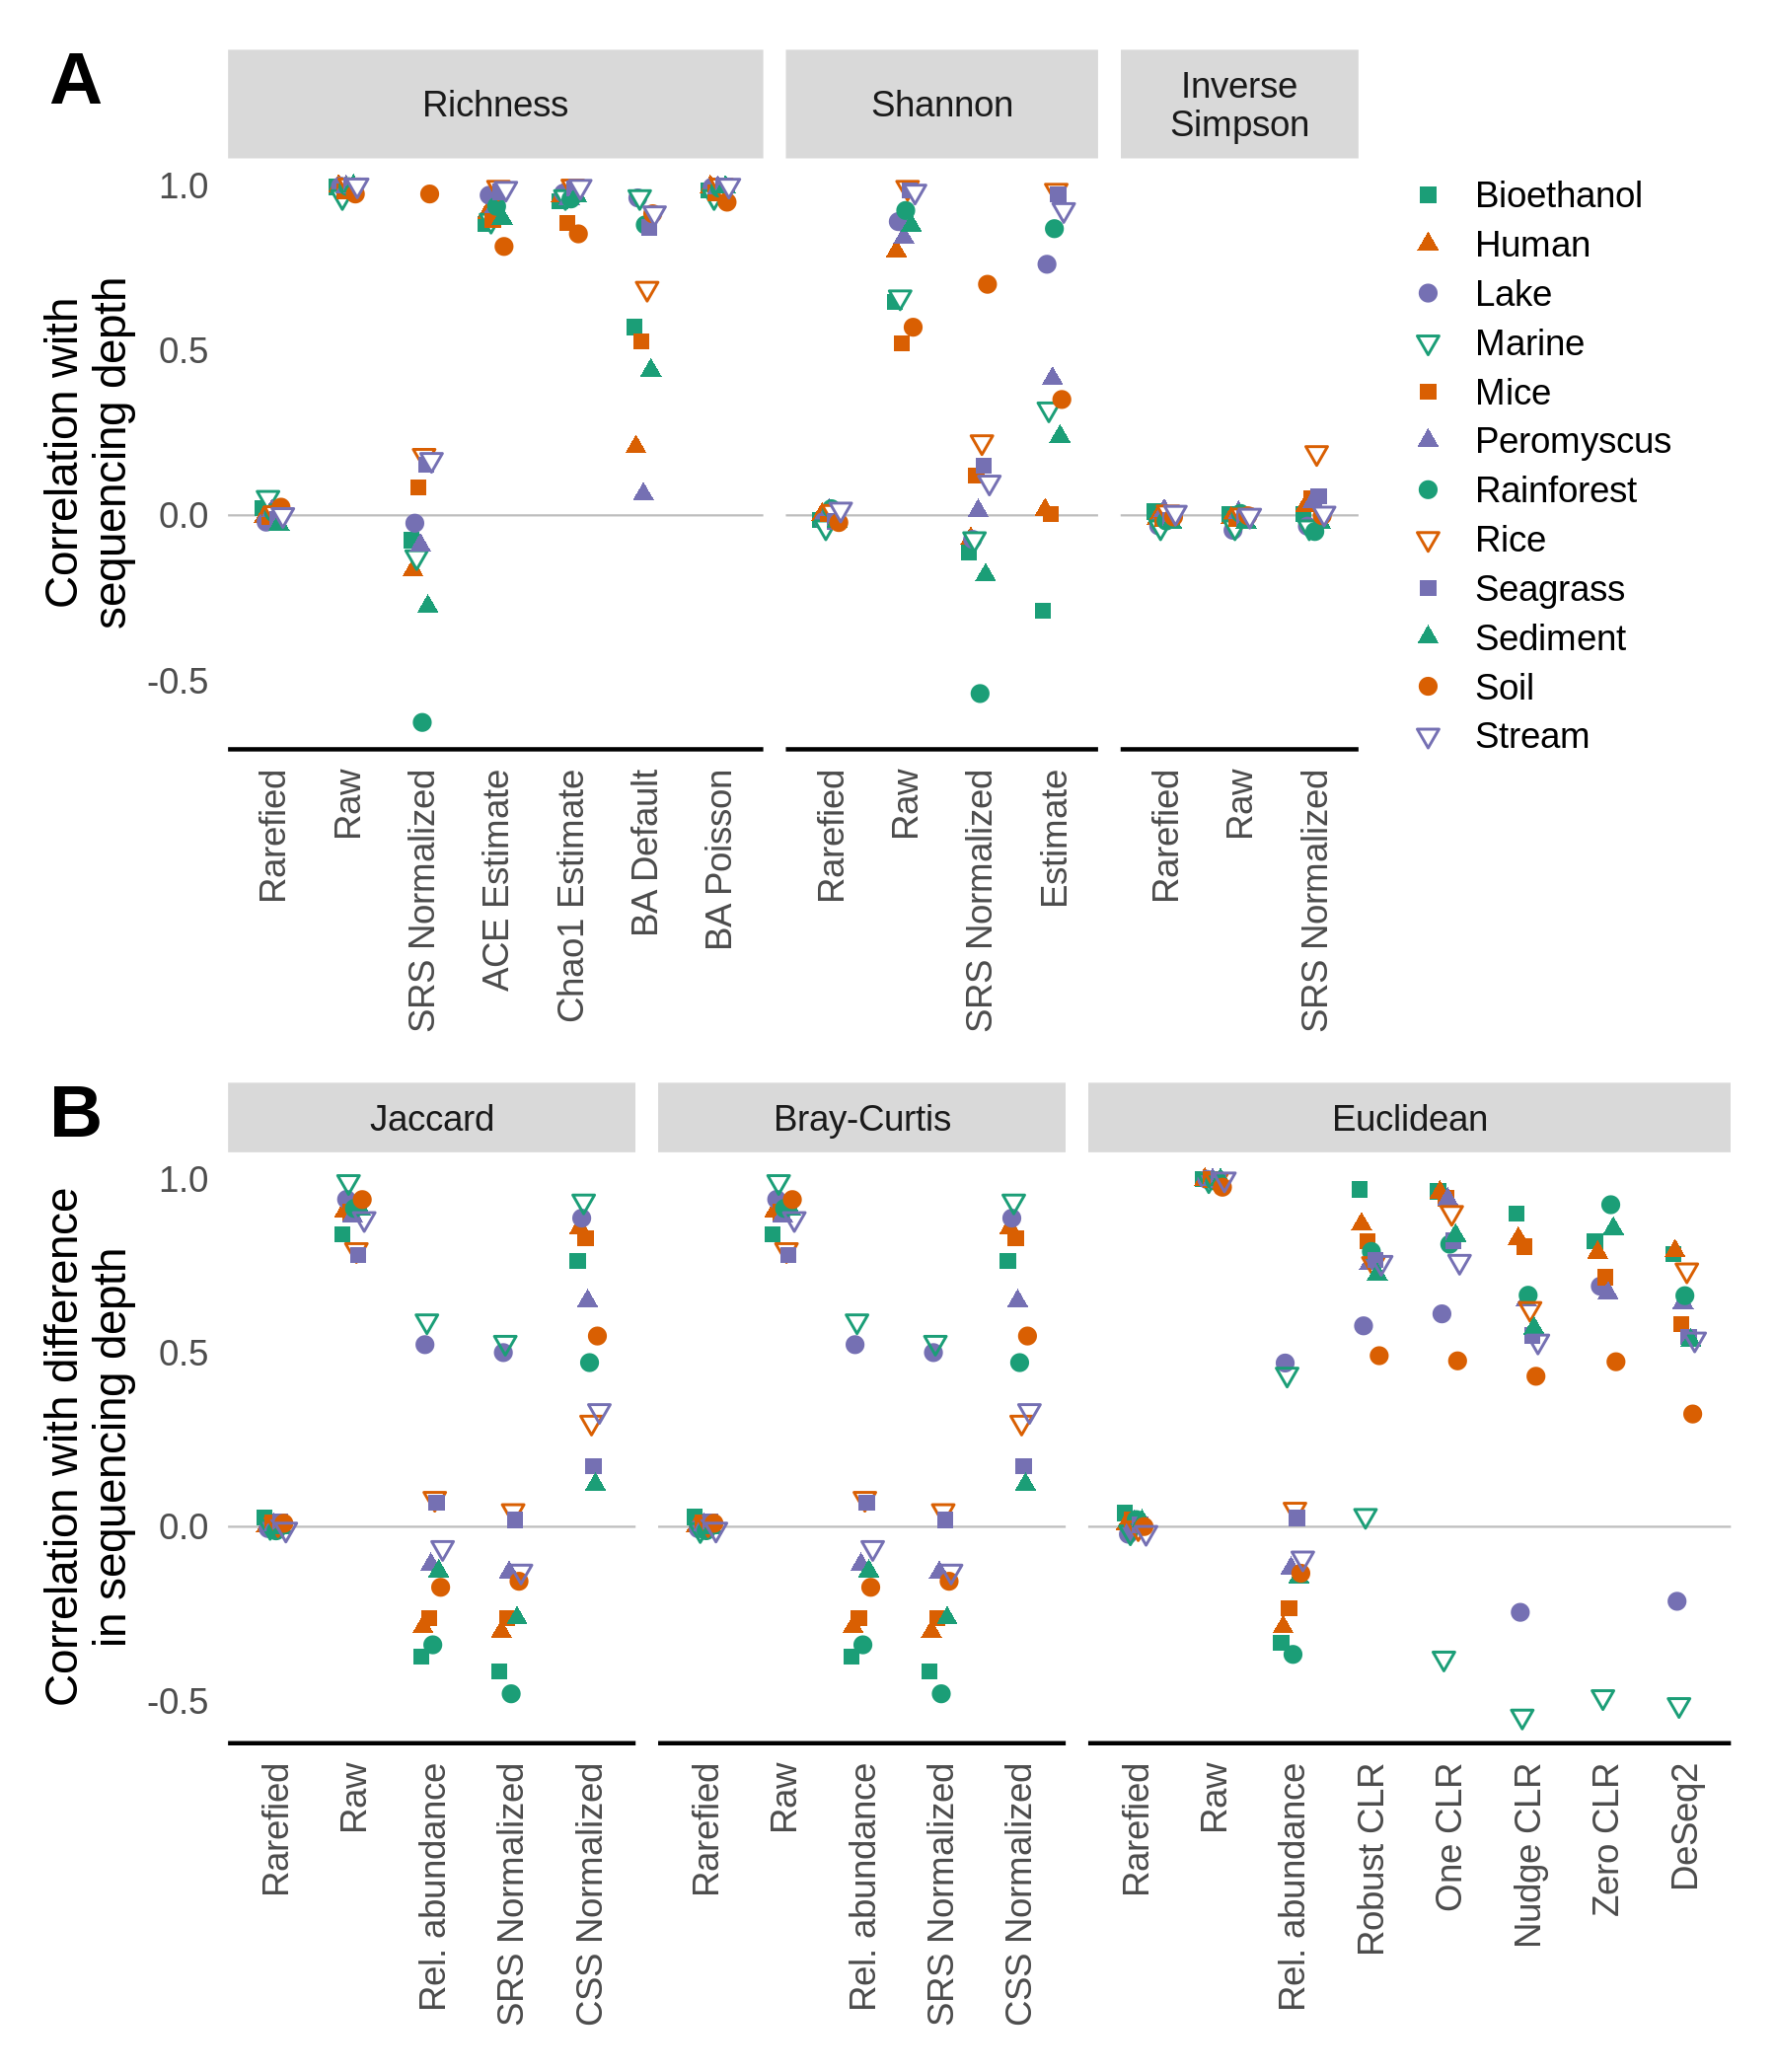
\includegraphics[height=17cm]{figure_1.png}

\textbf{Figure 1. Rarefaction eliminates the correlation between
sequencing depth and alpha diversity (A) and between differences in
sequencing depth and beta (B) diversity metrics when using null
community models.} Examples of the relationship between different
metrics and methods for controlling for uneven sequencing effort are
provided in Figures S2 and S3 for alpha and beta diversity metrics,
respectively. Each point represents the mean of 100 random null
community models; the standard deviation was smaller than the size of
the plotting symbol.

\newpage

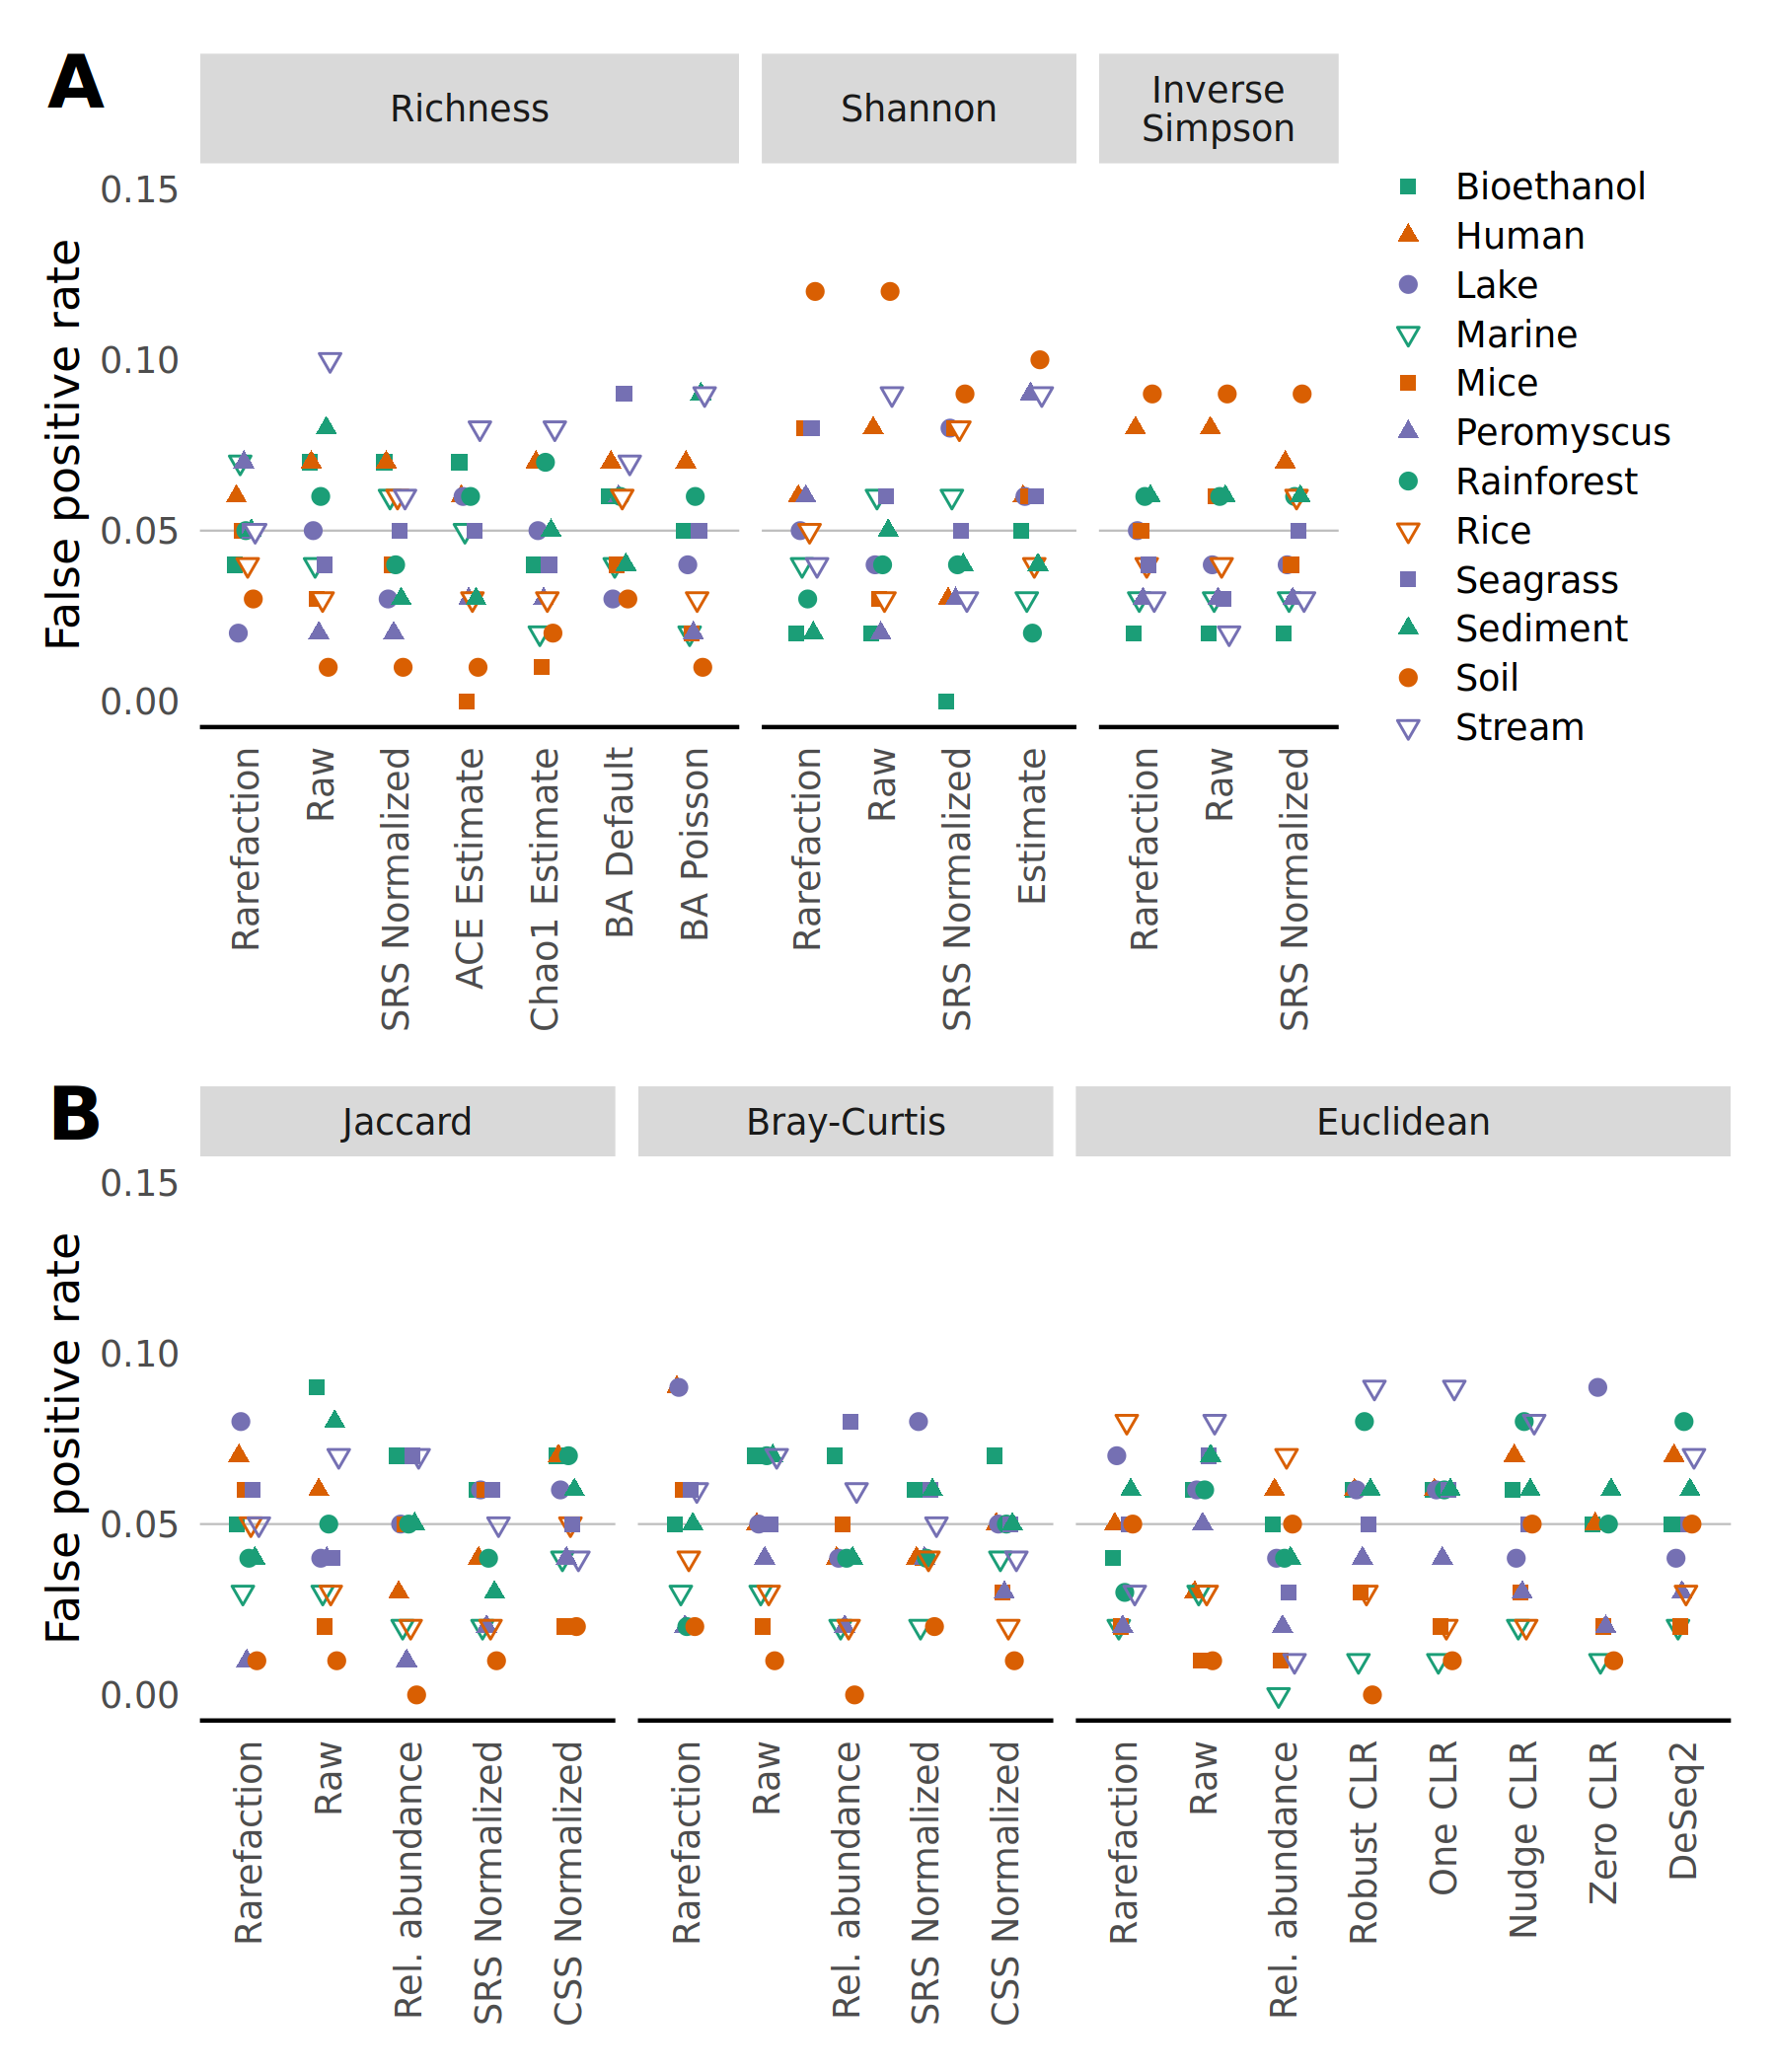
\includegraphics[height=17cm]{figure_2.png}

\textbf{Figure 2. The risk of falsely detecting a difference between
treatment groups drawn from a null model does not meaningfully vary from
5\%, regardless of approach for controlling for uneven sequencing
depth}. Samples were randomly assigned to different treatment groups. To
calculate the false detection rate, datasets were regenerated 100 times
and differences in alpha diversity were tested using a Wilcoxon test (A)
and differences in beta diversity were tested using PERMANOVA (B) at a
5\% threshold. The false positive rate was the number of times a dataset
yielded a significant result.

\newpage

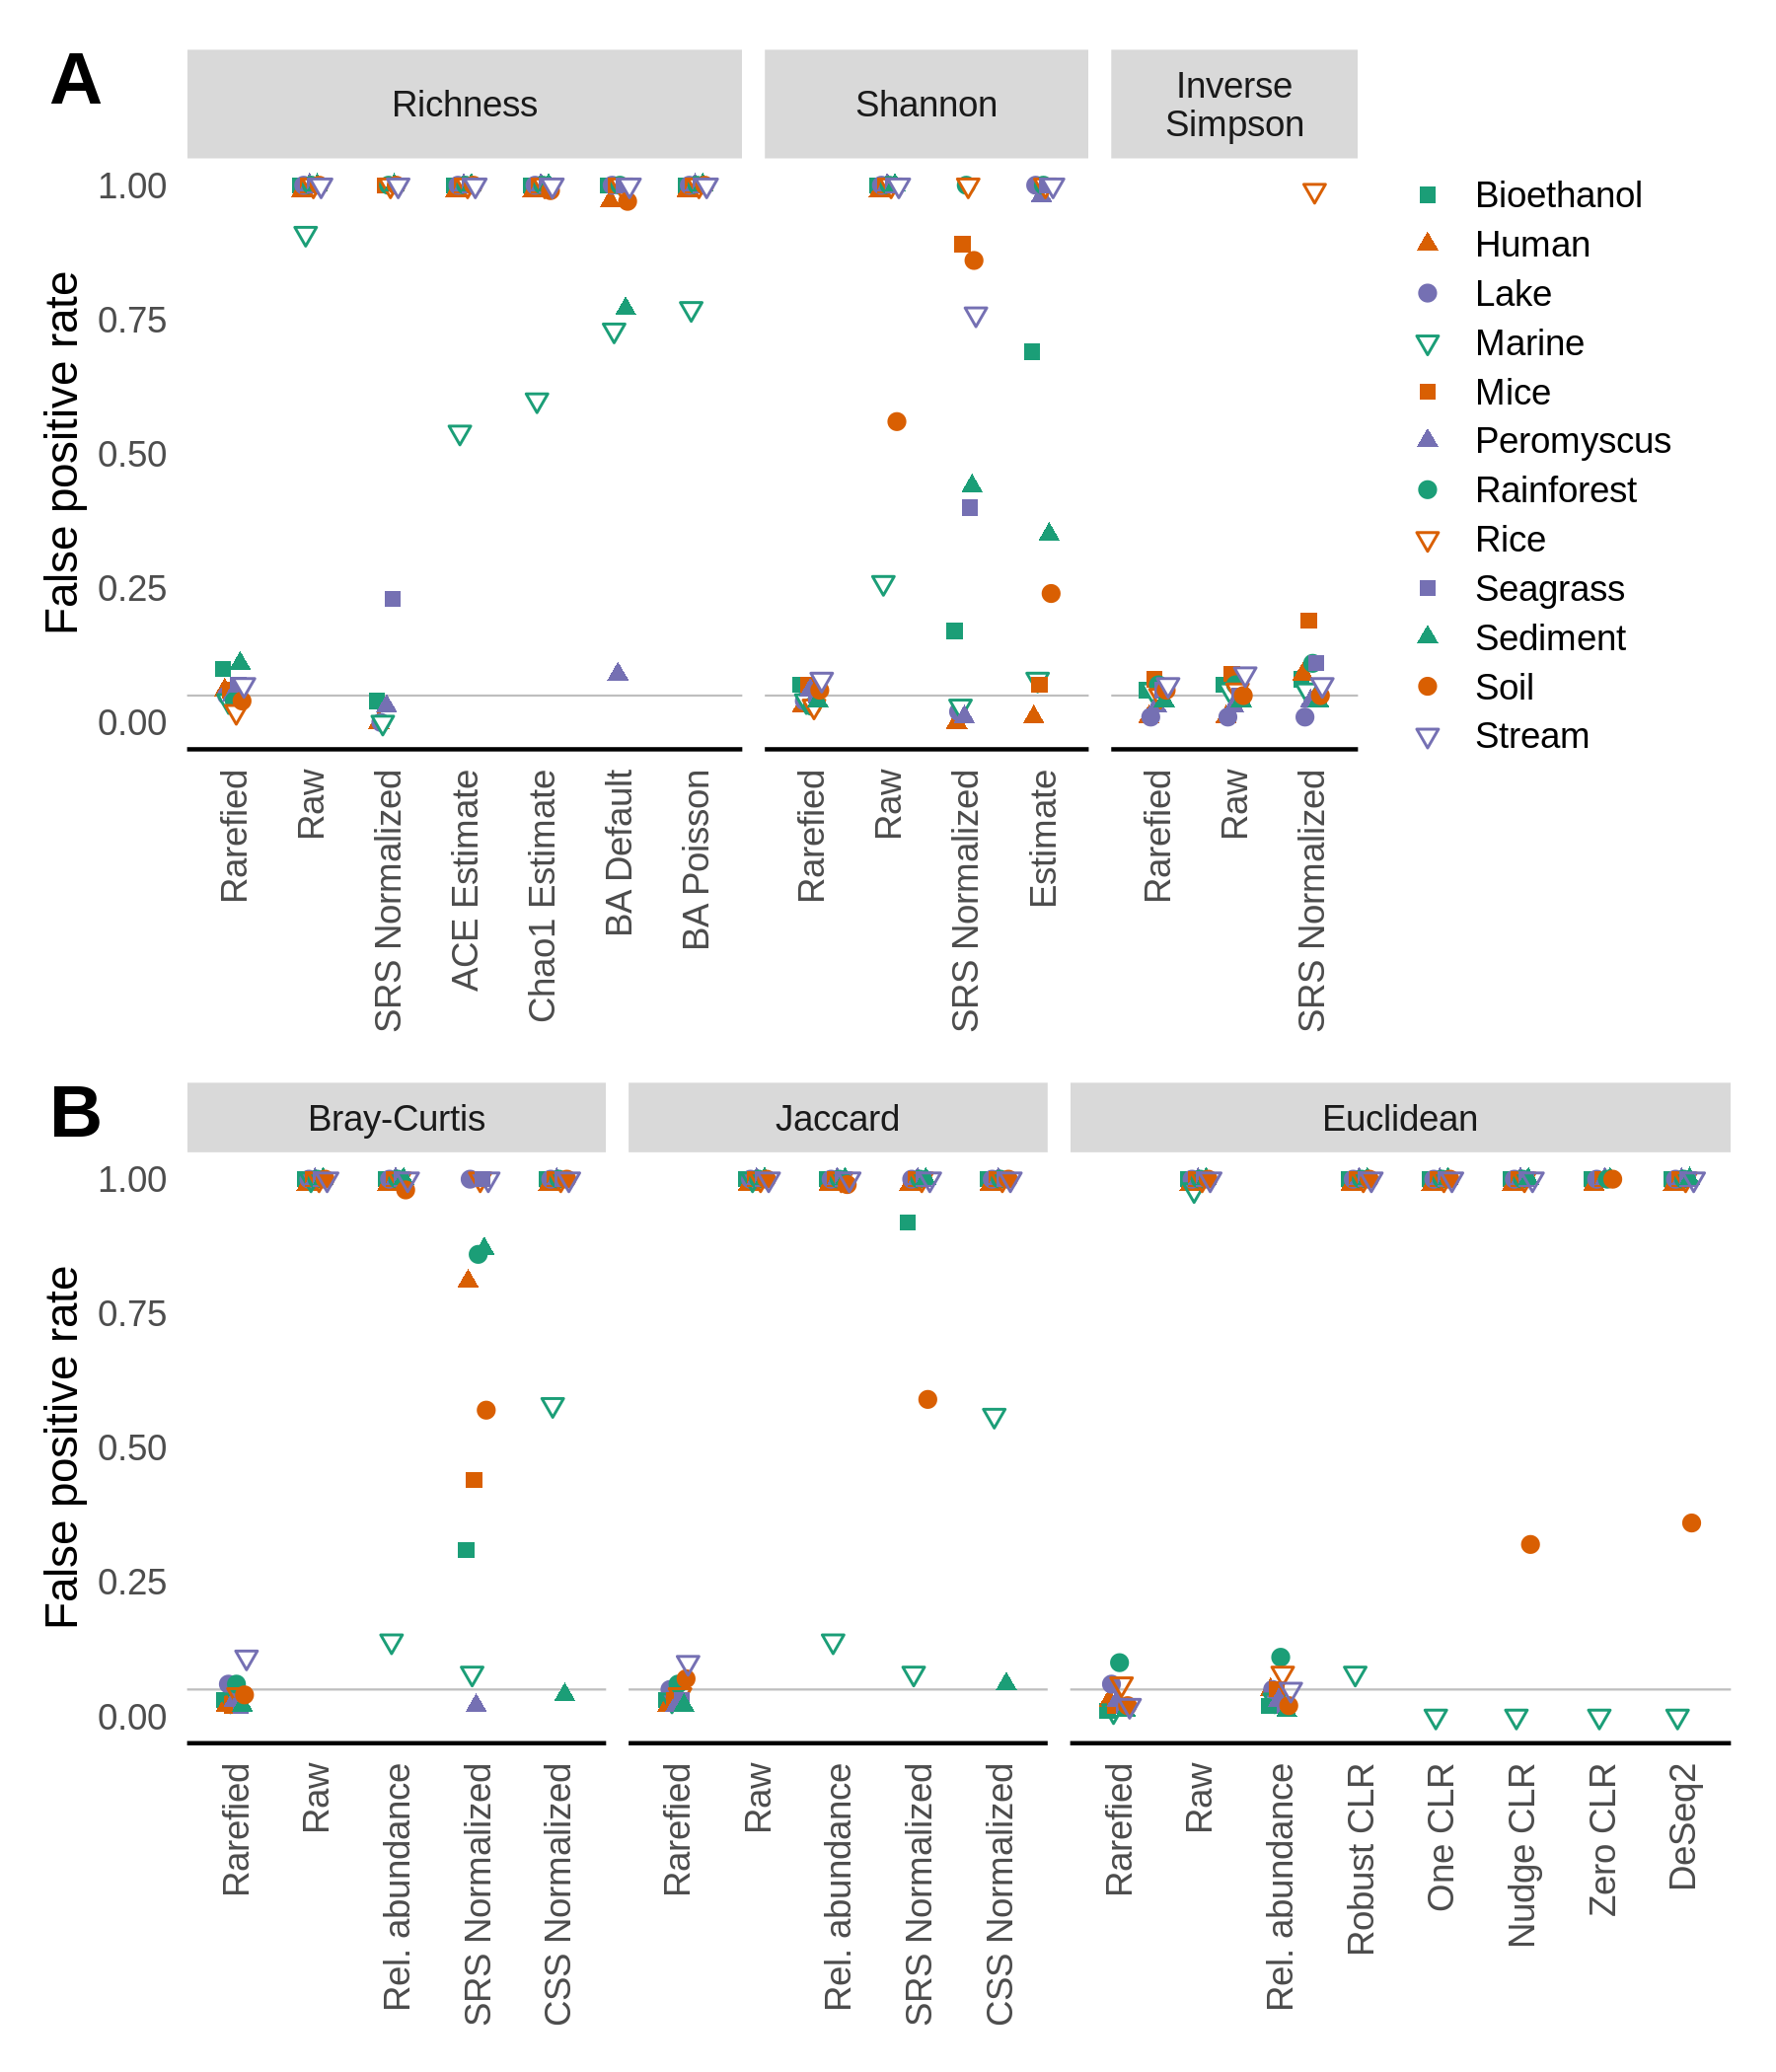
\includegraphics[height=17cm]{figure_3.png}

\textbf{Figure 3.The risk of falsely detecting a difference between
treatment groups drawn from a null model does not meaningfully vary from
5\% when data are normalized by rarefaction when sequencing depth is
confounded with treatment group}. Samples were assigned to different
treatment groups based on whether they were above the median number of
sequences for each dataset. To calculate the false detection rate,
datasets were regenerated 100 times and differences in alpha diversity
were tested using a Wilcoxon test (A) and differences in beta diversity
were tested using PERMANOVA (B) at a 5\% threshold. The false positive
rate was the number of times a dataset yielded a significant result.

\newpage

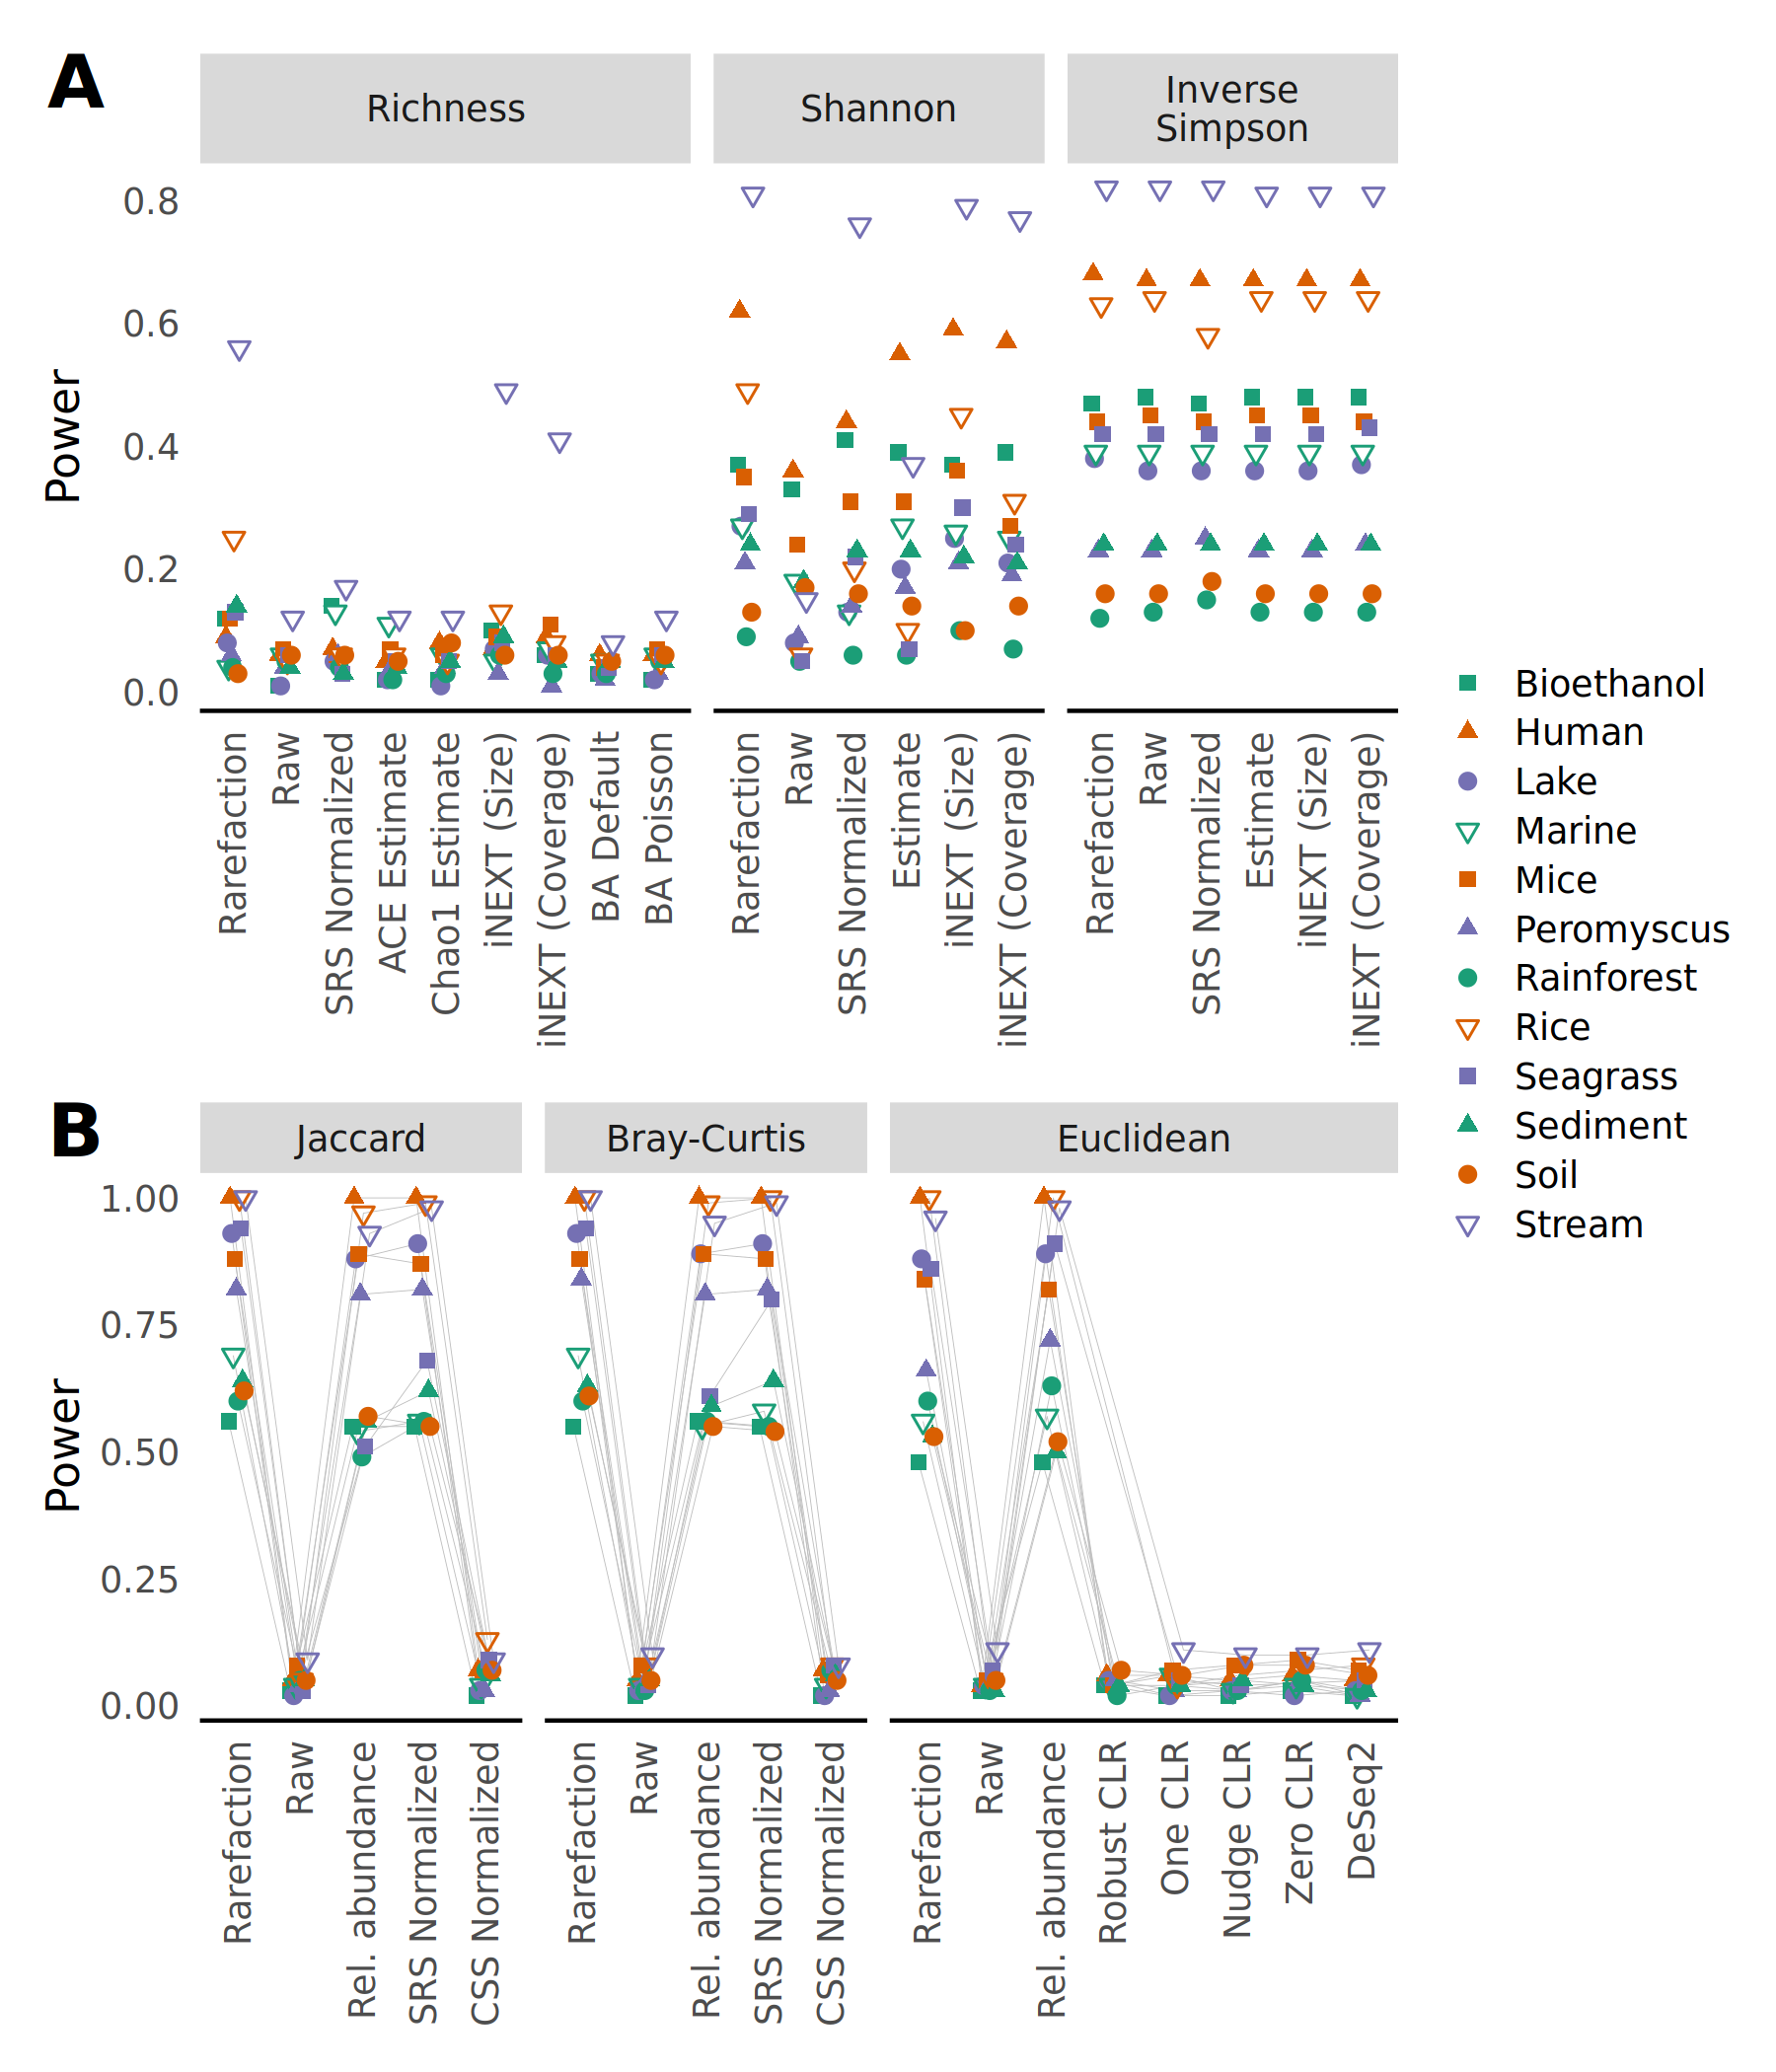
\includegraphics[height=17cm]{figure_4.png}

\textbf{Figure 4. The ability to detect true differences in treatment
groups for alpha (A) and beta (B) diversity metrics is greatest when
communities differing in the relative abundance of their OTUs are
normalized by rarefaction.} For each dataset samples were randomly
assigned to one of two community distributions where the abundance of
OTUs differed. To calculate the power for each datasets, datasets were
regenerated 100 times and differences in alpha diversity were tested
using a Wilcoxon test (A) and differences in beta diversity were tested
using PERMANOVA (B) at a 5\% threshold. The power was the number of
times a dataset yielded a significant result.

\newpage

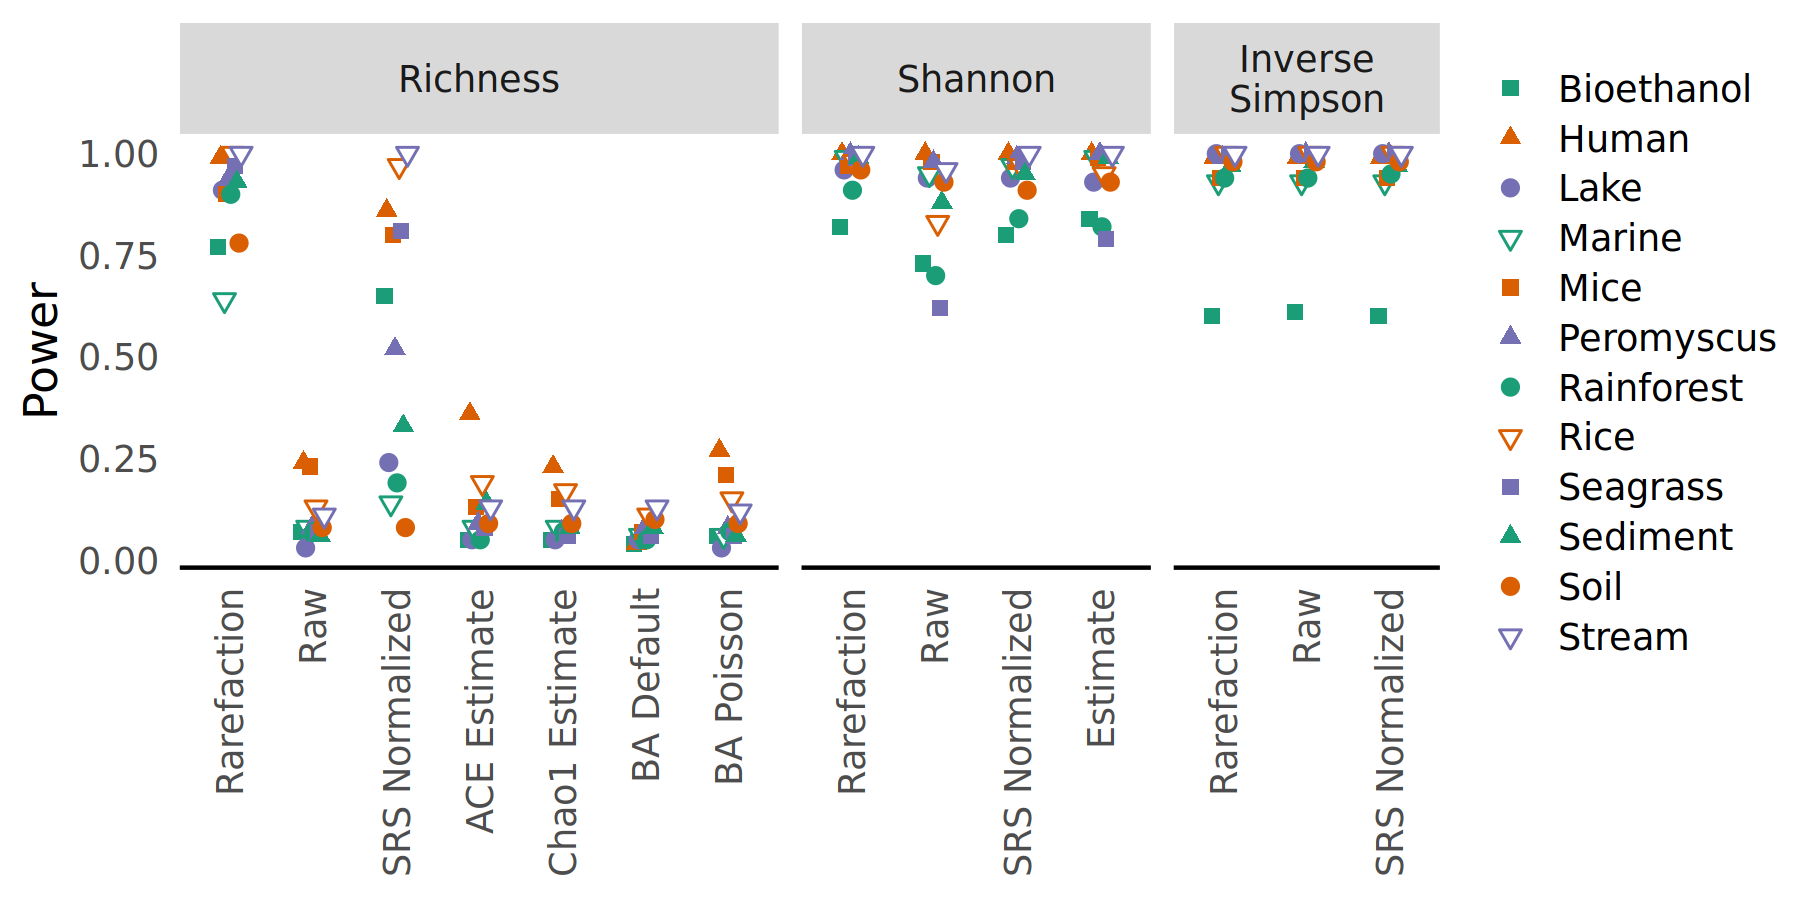
\includegraphics{figure_5.png}

\textbf{Figure 5. The ability to detect true differences in treatment
groups for alpha diversity metrics is greatest when sequencing depths
from communities differing in richness are normalized by rarefaction.}
For each dataset samples were randomly assigned to one of two community
distributions where one distribution contained a subset of OTUs found in
the other. To calculate the power for each dataset, datasets were
regenerated 100 times and differences in alpha diversity were tested
using a Wilcoxon test (A) and differences in beta diversity were tested
using PERMANOVA (B) at a 5\% threshold. The power was the number of
times a dataset yielded a significant result.

\newpage

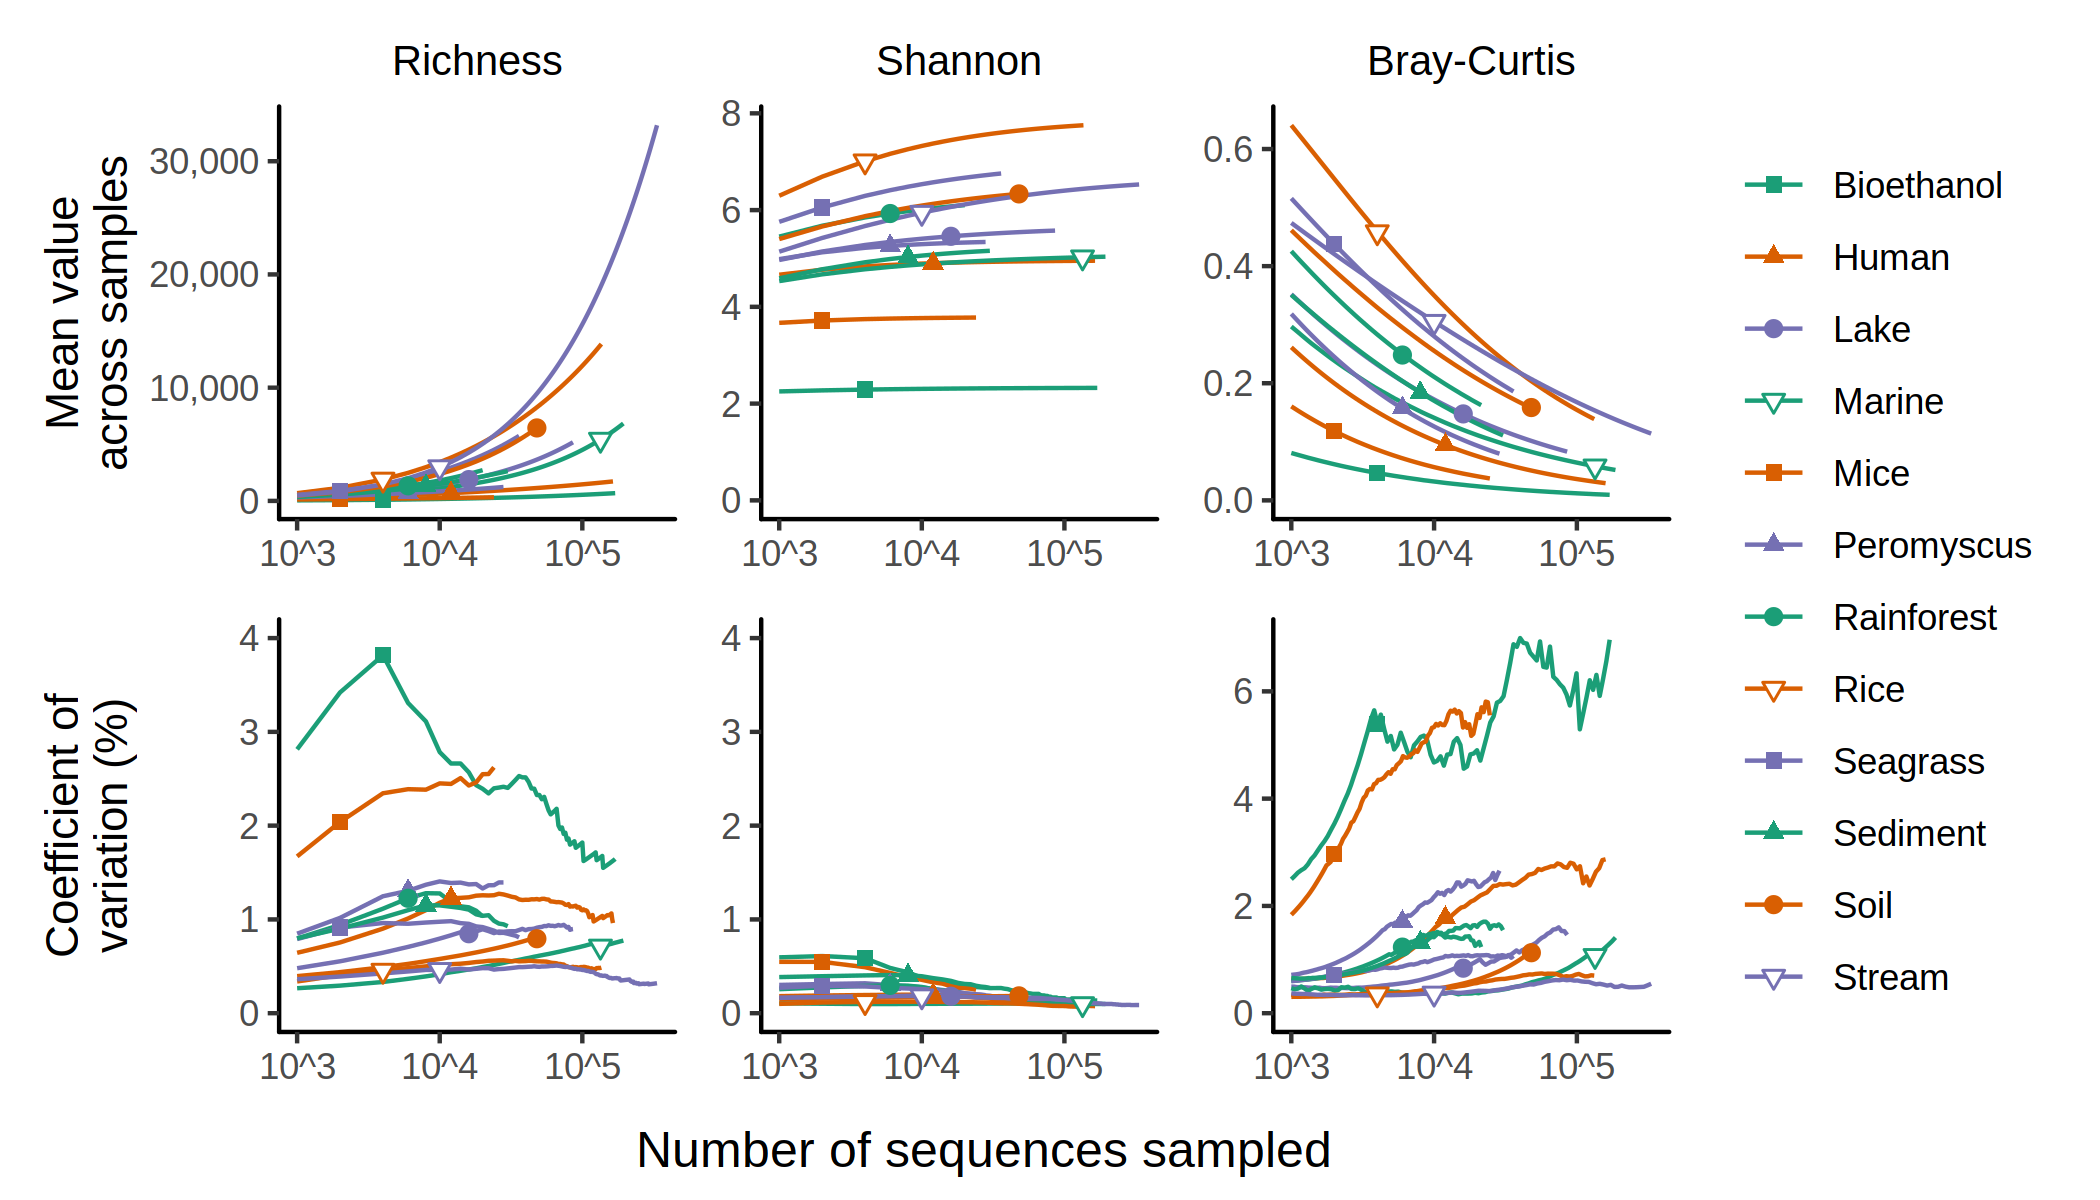
\includegraphics{figure_6.png}

\textbf{Figure 6. The mean and coefficient of variation for richness,
Shannon diversity, and Bray-Curtis dissimilarity values calculated by
rarefaction vary with sequencing depth.} For each dataset, a null
community distribution was created and samples were created to have the
same sequencing depth as they did originally. The placement of the
plotting symbol indicates the size of the smallest sample. Results are
only shown for sequencing depths where a dataset had 5 or more samples.

\newpage

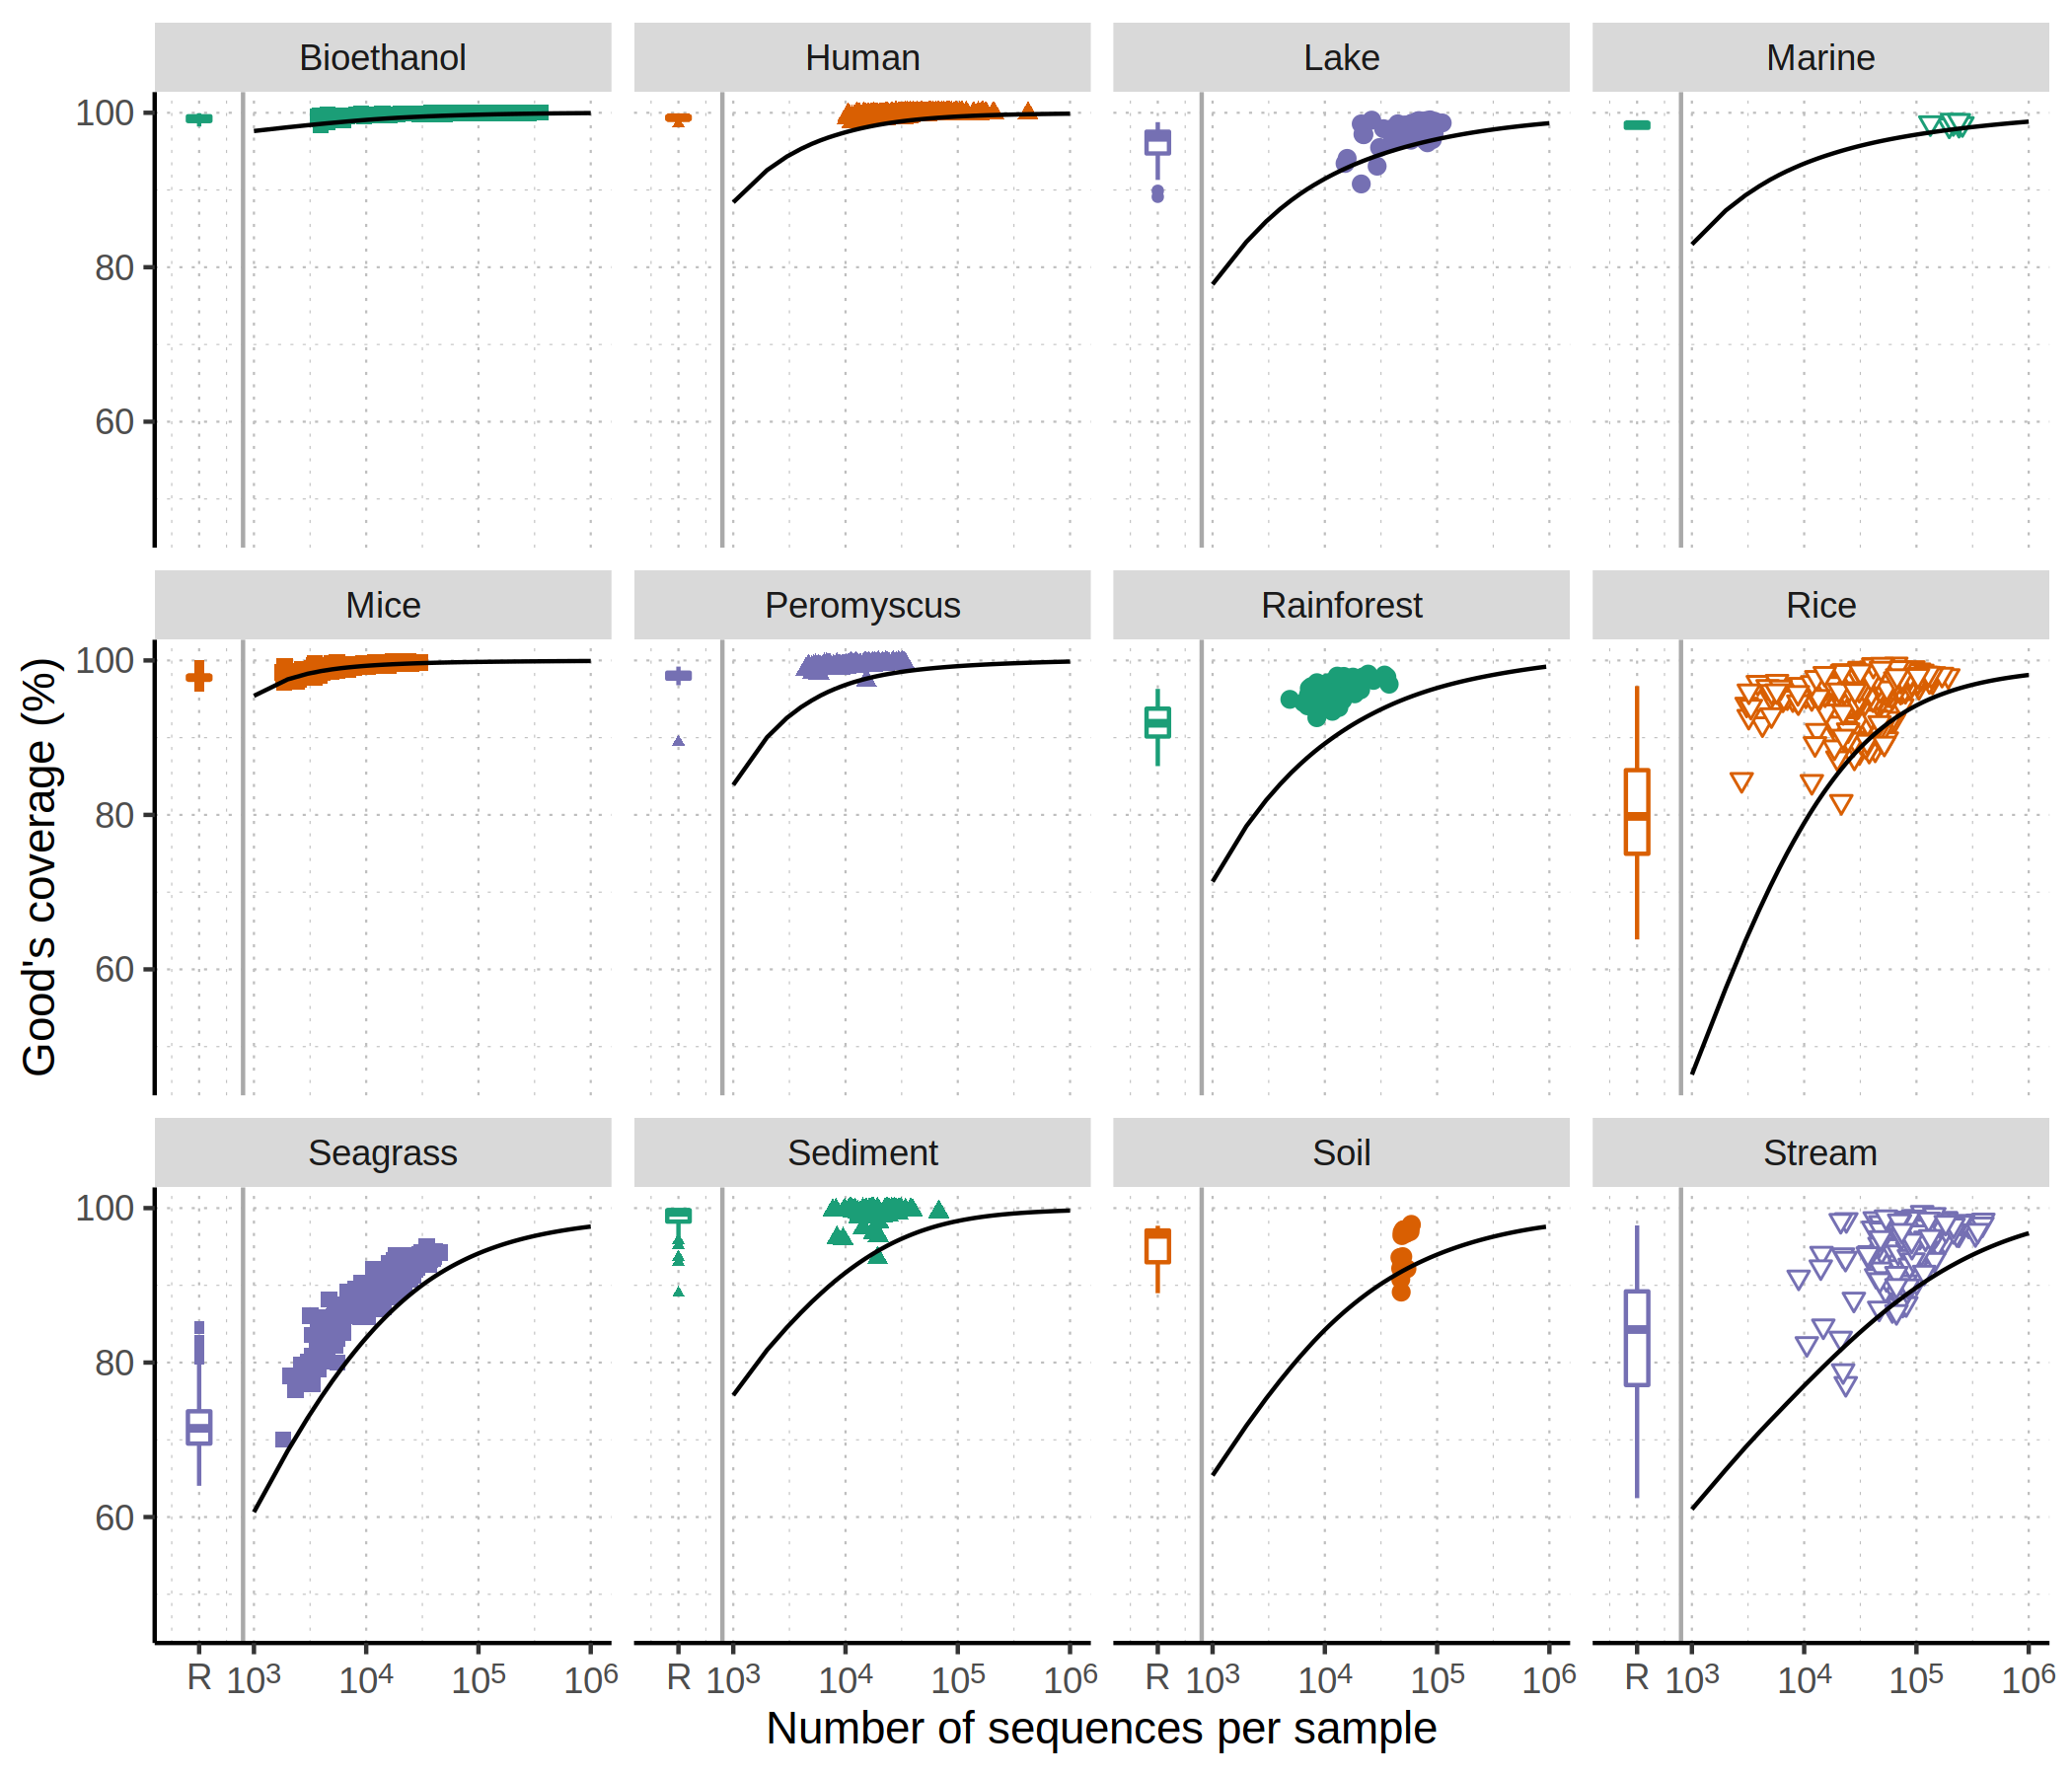
\includegraphics{figure_7.png}

\textbf{Figure 7. Most datasets are sequenced to a level that provides a
high level of coverage.} Each plotting symbol represents the observed
Good's coverage for a different sample in each dataset. The smoothed
line indicates the simulated coverage for varying levels of sequencing
effort when a null community is generated from the observed data. The
box and whisker plot indicates the range of coverage values when the
observed community data were normalized by rarefaction to the size of
the least sequenced sample.

\newpage

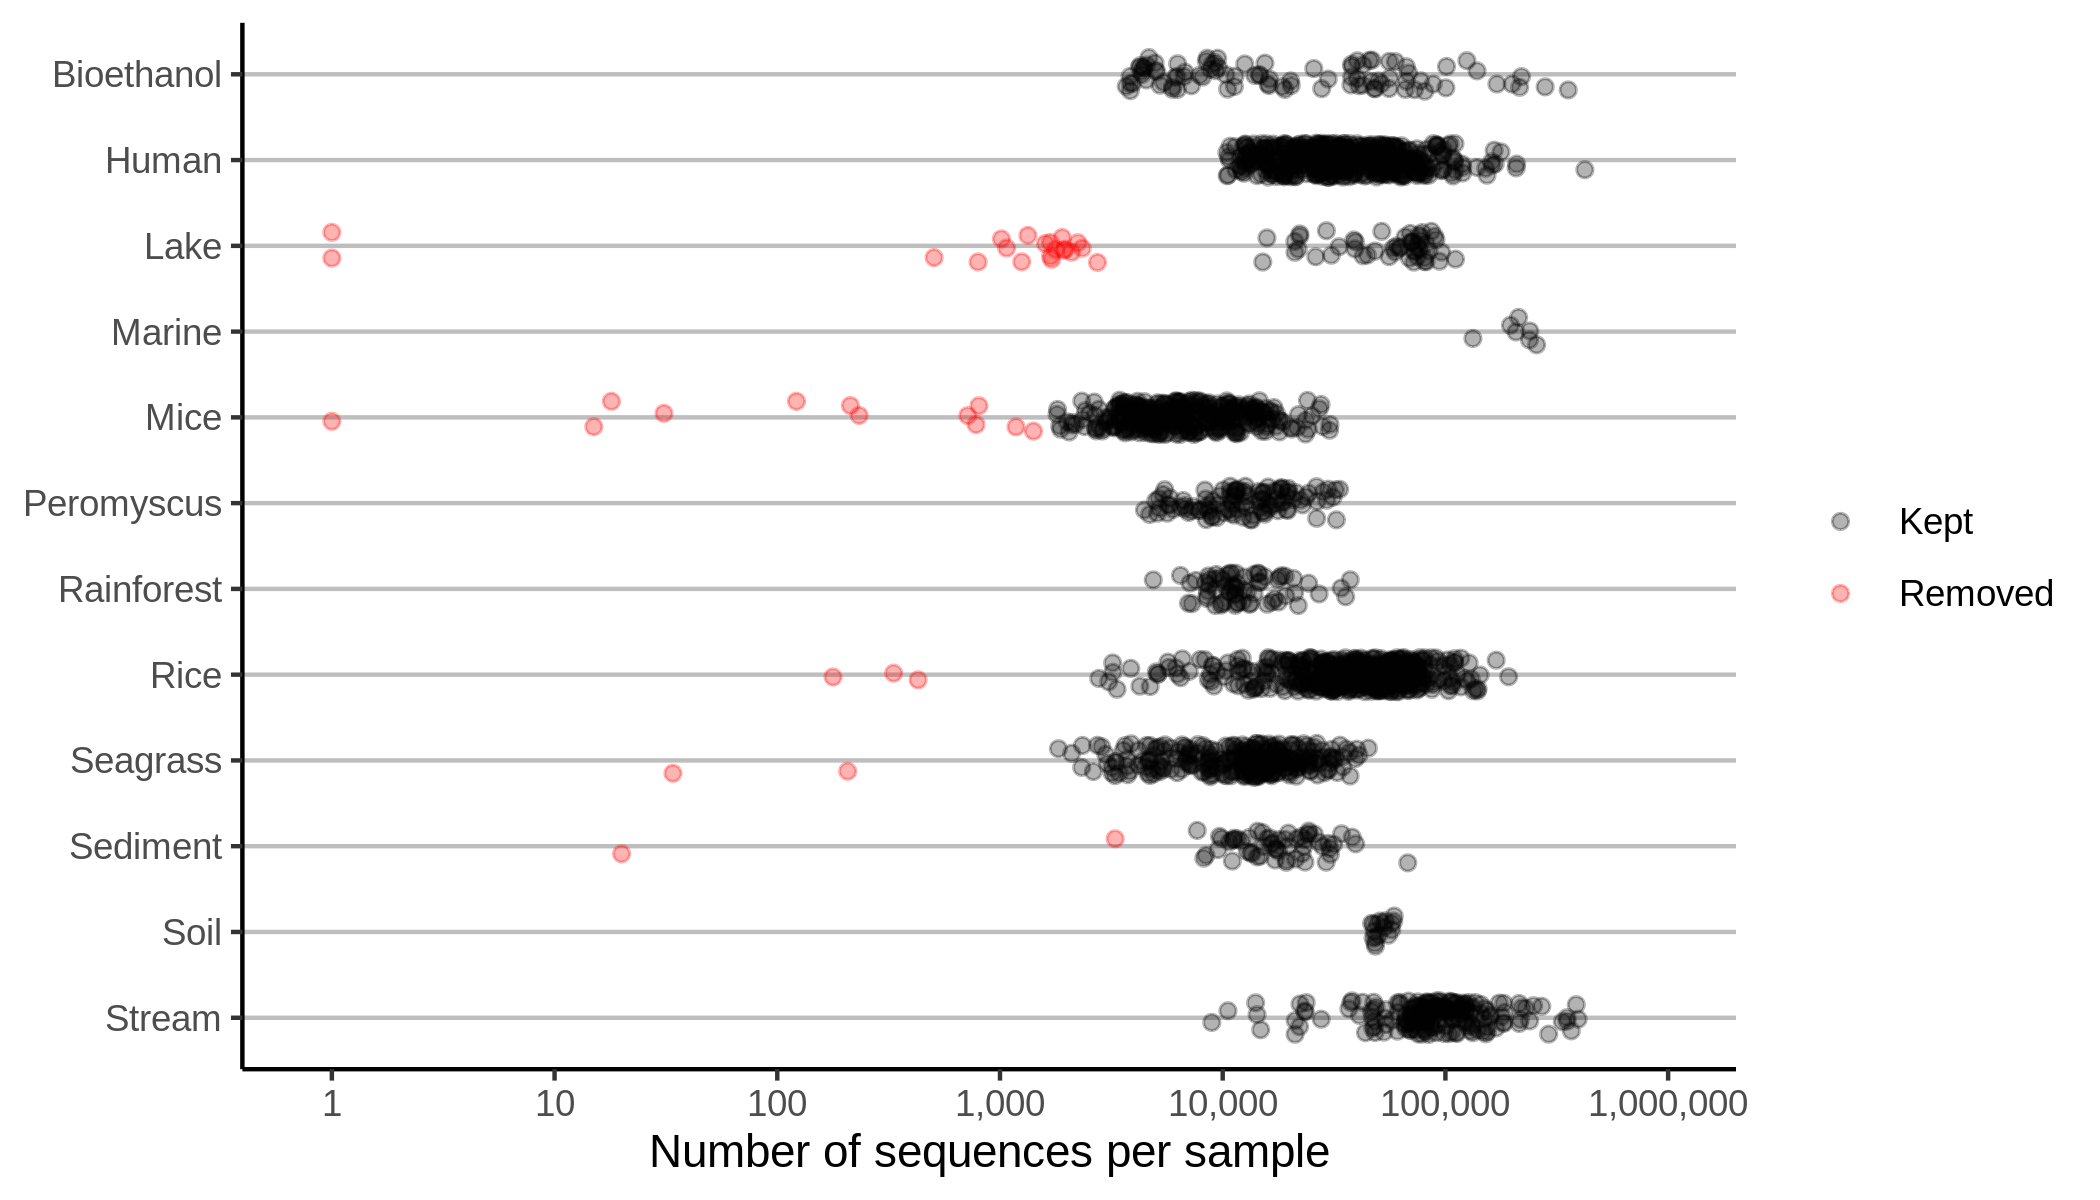
\includegraphics{figure_s1.png}

\textbf{Figure S1. The number of sequences observed in each sample for
each dataset included in this analysis generally varied by 10 to
100-fold.} The threshold for specifying the number of sequences per
sample varied by dataset and was determined based on identifying natural
breaks in the data. This figure is similar to Figure S1 of (27)

\newpage

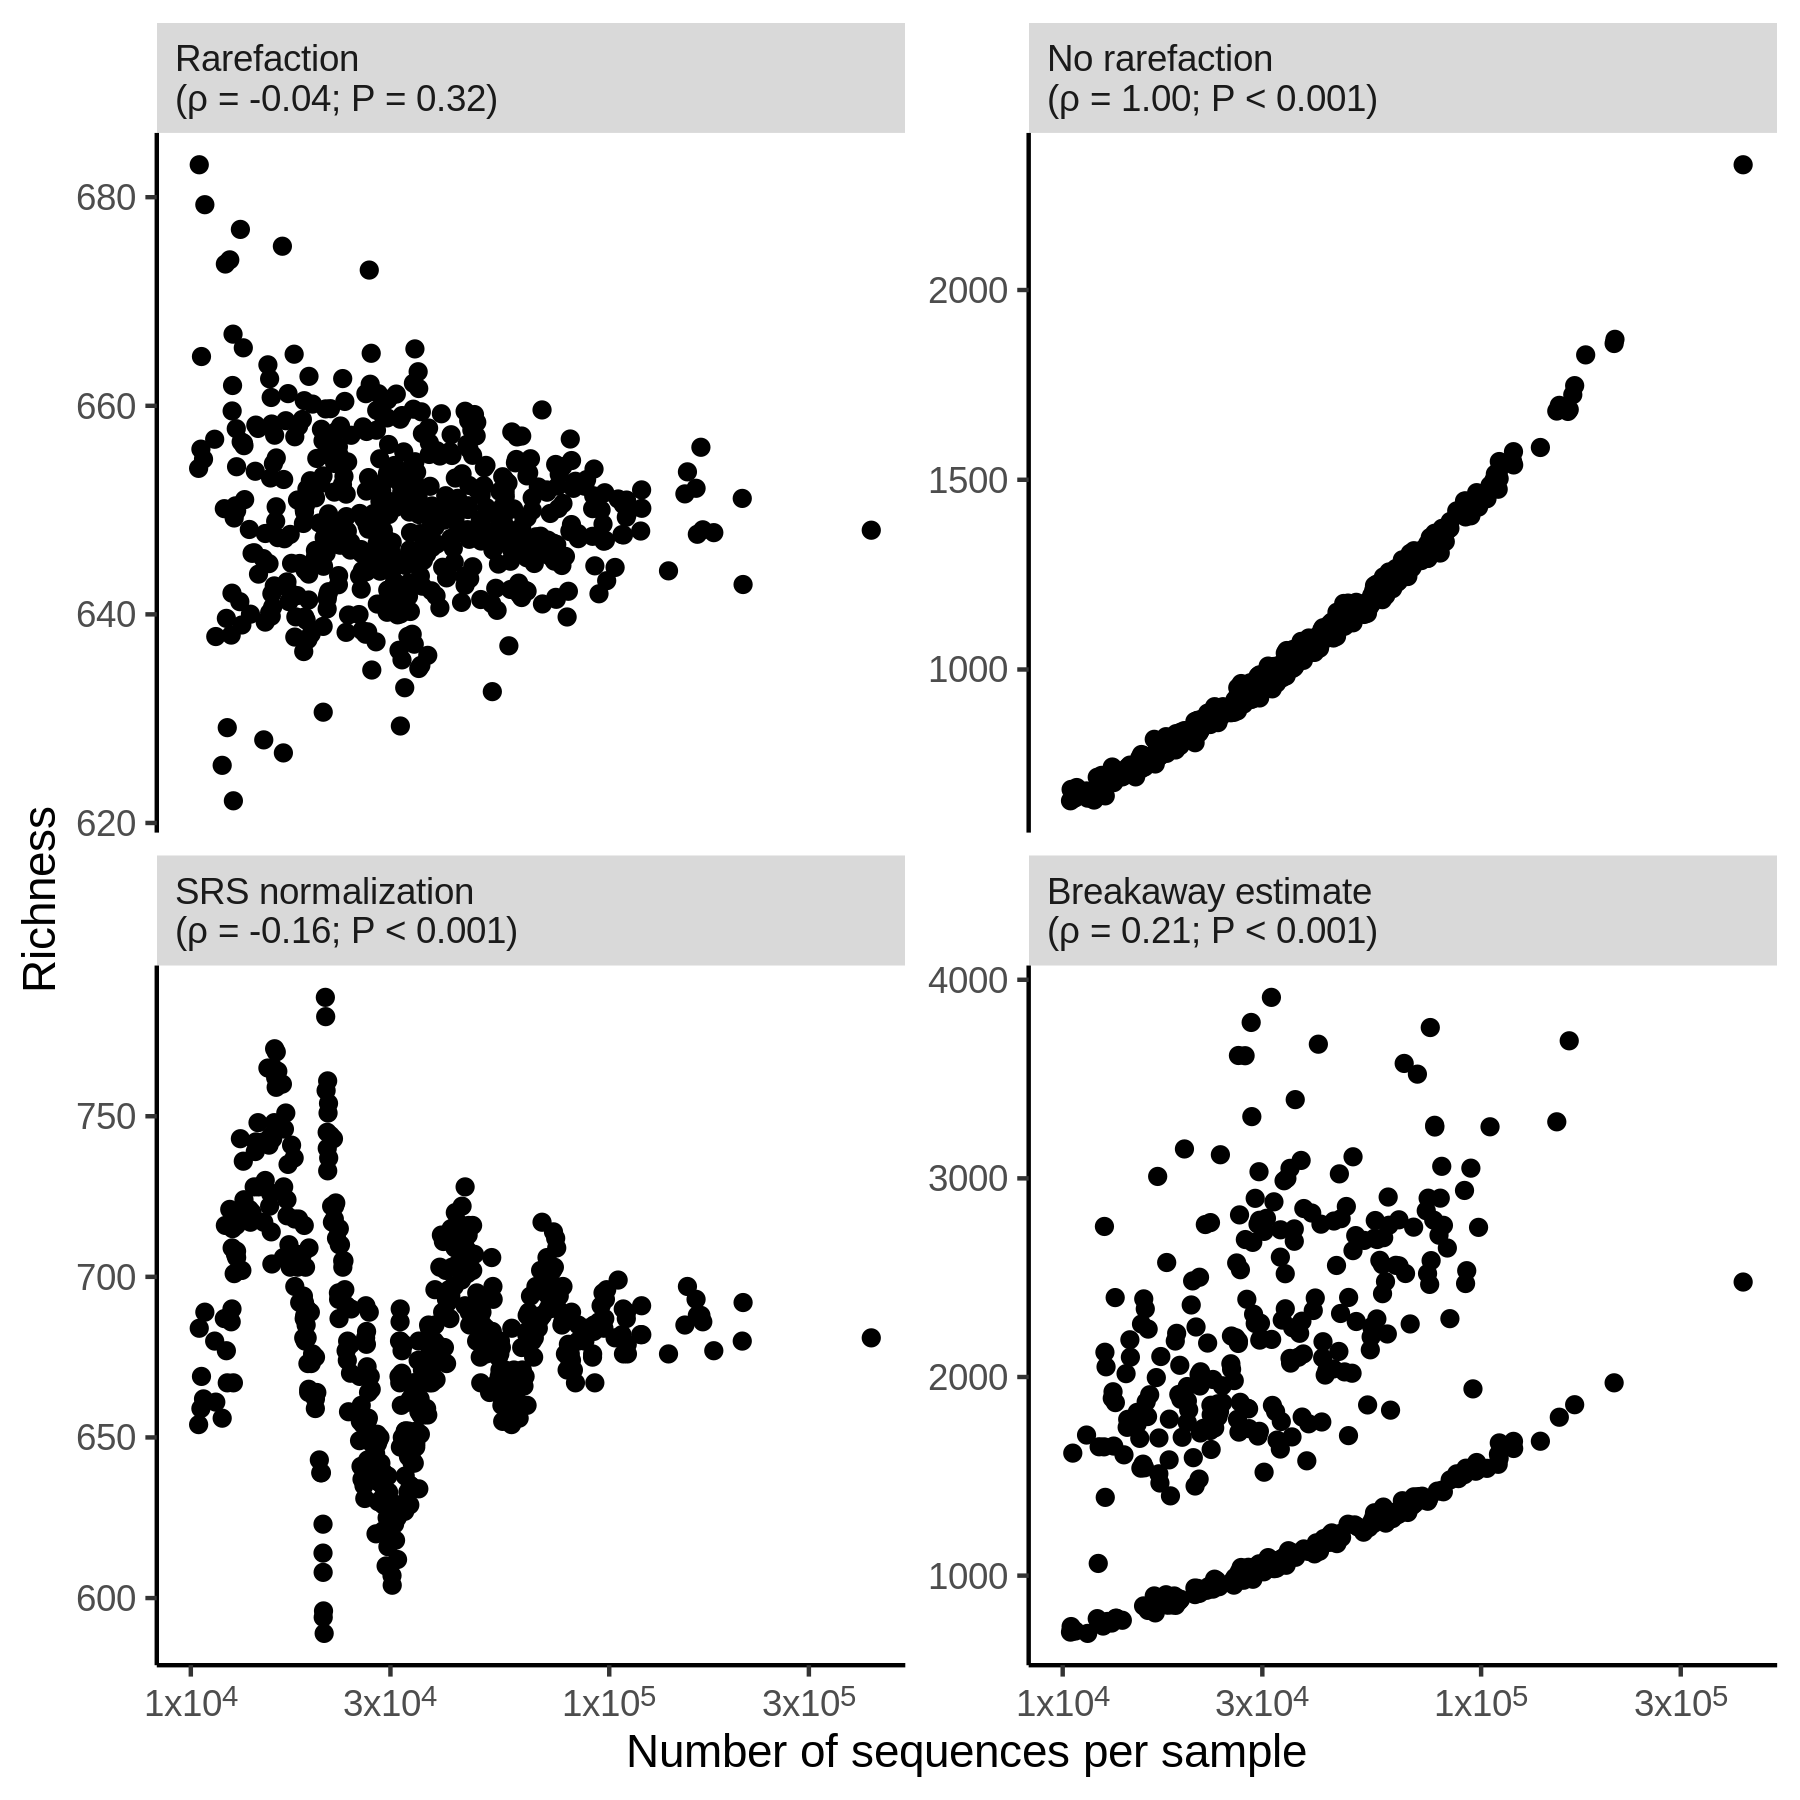
\includegraphics{figure_s2.png}

\textbf{Figure S2. Examples of the richness in each of the 490 samples
that were generated for one randomization of the null model using the
human dataset.} The x-axis indicates the number of sequences in each of
the samples prior to each method's approach of controlling for uneven
sequencing effort. The Spearman correlation coefficient (\(\rho\)) and
test of whether the coefficient was significantly different from zero
are indicated for each panel.

\newpage

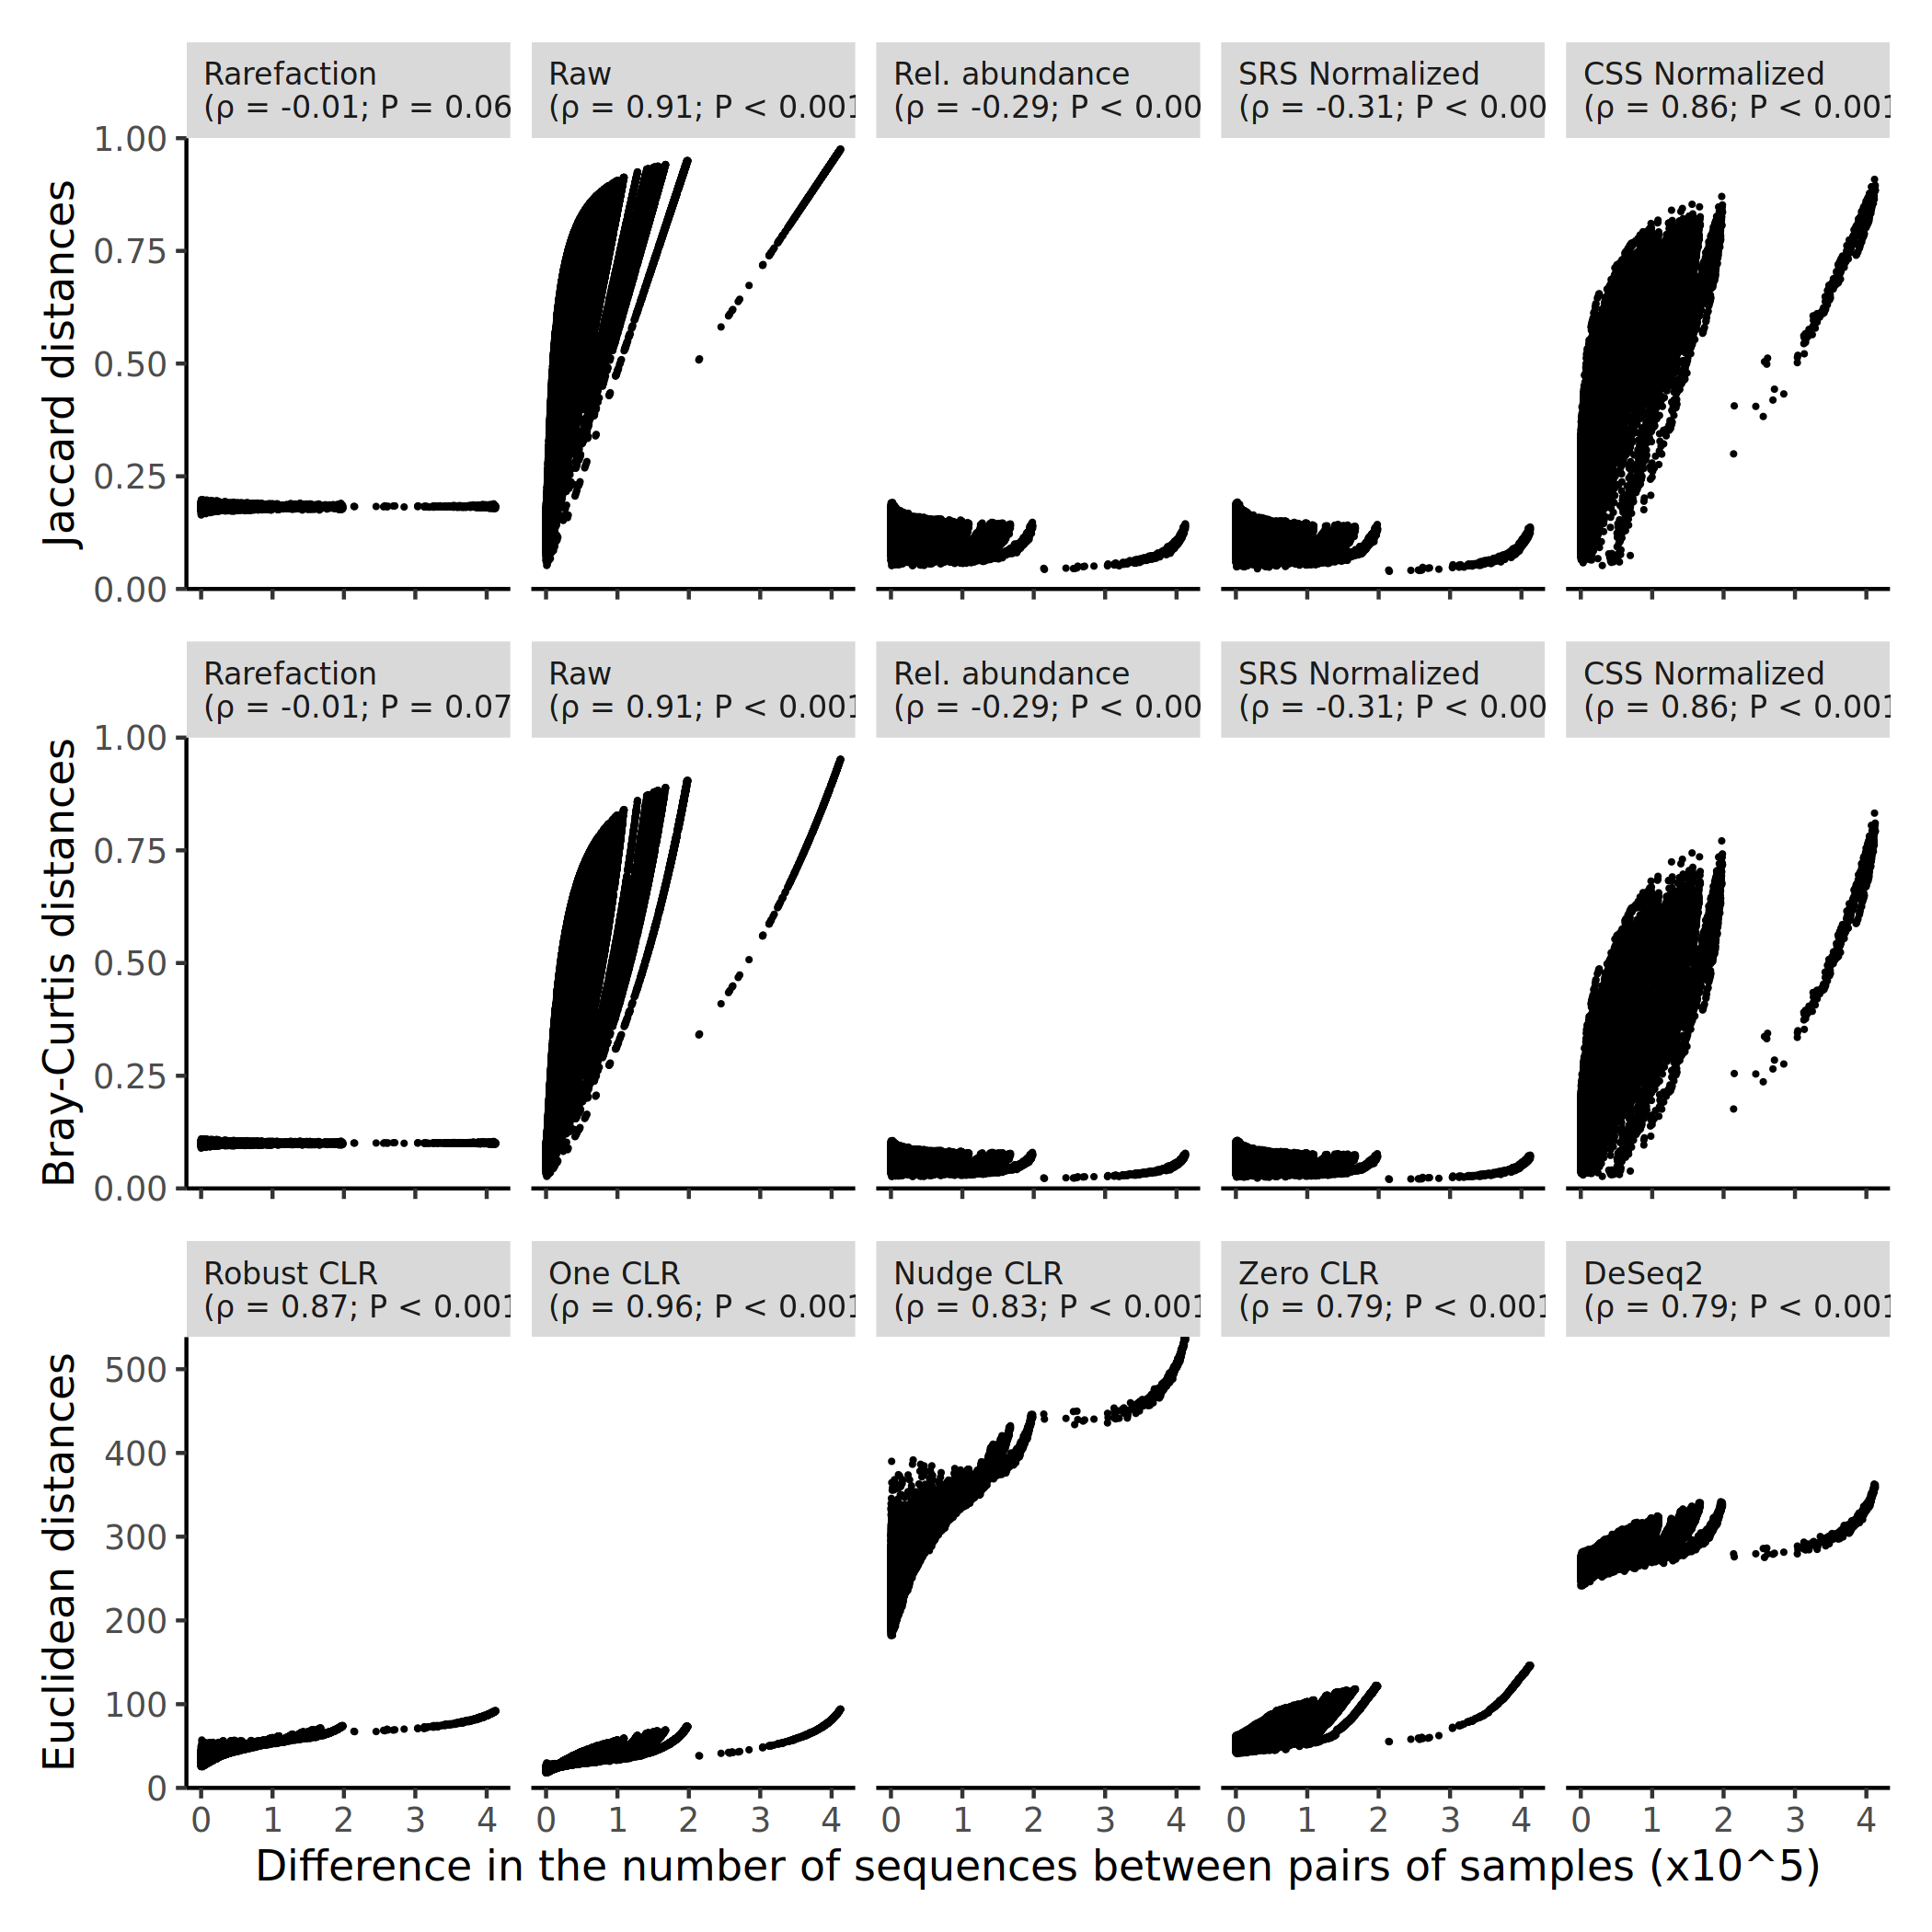
\includegraphics{figure_s3.png}

\textbf{Figure S3. Examples of differences in beta diversity in each of
the 490 samples that were generated for one randomization of the null
model using the human dataset.} The x-axis indicates the difference in
the number of sequences in each of the samples that went into
calculating the pairwise distance prior to each method's approach of
controlling for uneven sequencing effort. The Spearman correlation
coefficient (\(\rho\)) and test of whether the coefficient was
significantly different from zero are indicated for each panel.

\end{document}
